%==========================================================================
% Chapter 8: Routing Algorithms
% Nature Inspired Optimisation for Delivery Problems (Urquhart, 2022)
% Self-contained lecture notes as Beamer slides
%==========================================================================
\documentclass[aspectratio=169,10pt]{beamer}

\usetheme{Madrid}
\usecolortheme{seahorse}

\usepackage{amsmath,amssymb}
\usepackage{booktabs}
\usepackage{xcolor}
\usepackage{listings}
\usepackage{graphicx}
\usepackage{tikz}
\usepackage{microtype}
\usepackage{hyperref}
\usepackage{array}
\usepackage{multirow}
\usepackage{colortbl}
\usepackage{caption}

\graphicspath{{figures/}}

\setbeamertemplate{footline}[frame number]
\setbeamertemplate{navigation symbols}{}

% --- listings style for Java/pseudocode ---
\lstdefinestyle{javacode}{
  language=Java,
  basicstyle=\ttfamily\scriptsize,
  numbers=left,
  numberstyle=\tiny\color{gray},
  frame=single,
  backgroundcolor=\color{gray!7},
  keywordstyle=\color{blue!70}\bfseries,
  commentstyle=\color{green!50!black}\itshape,
  stringstyle=\color{orange!80!black},
  breaklines=true,
  tabsize=2,
  xleftmargin=1.5em,
  framexleftmargin=1.5em,
  showstringspaces=false,
}

% --- listings style for pseudocode ---
\lstdefinestyle{pseudocode}{
  basicstyle=\ttfamily\scriptsize,
  numbers=left,
  numberstyle=\tiny\color{gray},
  frame=single,
  backgroundcolor=\color{blue!4},
  keywordstyle=\color{blue!80}\bfseries,
  commentstyle=\color{green!50!black}\itshape,
  breaklines=true,
  tabsize=2,
  xleftmargin=1.5em,
  framexleftmargin=1.5em,
  morekeywords={Procedure,EndProcedure,while,do,for,if,then,return,Return},
}

% --- listings style for Python ---
\lstdefinestyle{pythoncode}{
  language=Python,
  basicstyle=\ttfamily\scriptsize,
  numbers=left,
  numberstyle=\tiny\color{gray},
  frame=single,
  backgroundcolor=\color{gray!7},
  keywordstyle=\color{blue!70}\bfseries,
  commentstyle=\color{green!50!black}\itshape,
  stringstyle=\color{orange!80!black},
  breaklines=true,
  tabsize=4,
  xleftmargin=1.5em,
  framexleftmargin=1.5em,
  showstringspaces=false,
}

\title[Chapter 8: Routing Algorithms]{%
  Chapter 8: Routing Algorithms}
\subtitle{Nature Inspired Optimisation for Delivery Problems}
\author{N.~Urquhart \\ \small{Lecture slides -- self-contained reading version}}
\date{2022}
\institute{Natural Computing Series, Springer}

%==========================================================================
\begin{document}
%==========================================================================

\begin{frame}
  \titlepage
\end{frame}

%--------------------------------------------------------------------------
\begin{frame}{Chapter Overview}
%--------------------------------------------------------------------------
  In order to solve real-world delivery and routing problems, we need a
  method for finding routes through road networks.  This chapter provides
  that foundation: it explains how geospatial data can be represented as
  a graph, and then surveys a range of algorithms that search that graph
  for the shortest path between two nodes.

  \medskip
  The chapter covers four main topics.

  \begin{enumerate}
    \item \textbf{Section 8.1 --- Routing Algorithms}: the core algorithms
      (Dijkstra and A*), their pseudocode, and step-by-step worked examples.
    \item \textbf{Section 8.2 --- A Comparison of Basic Search Algorithms}:
      how the algorithms perform on real road networks (Sirmione, Italy and
      Edinburgh, UK), with timing data and statistical analysis.
    \item \textbf{Section 8.3 --- Hierarchical Structures}: how splitting
      the road graph by road type (motorway, primary, residential) enables
      much faster routing on large networks.
    \item \textbf{Section 8.4 --- Conclusions}: summary and implications for
      delivery-problem solvers.
  \end{enumerate}

  \begin{alertblock}{Why routing algorithms matter for delivery problems}
    Every time a solver proposes a sequence of customer visits, the routing
    engine must convert that abstract sequence into an actual road distance.
    Without an efficient routing algorithm, the solver would be crippled by
    the time spent computing distances.
  \end{alertblock}
\end{frame}

%==========================================================================
\section{8.1 Routing Algorithms}
%==========================================================================

%--------------------------------------------------------------------------
\begin{frame}[allowframebreaks]{Graphs as Road Networks}
%--------------------------------------------------------------------------
  A \textbf{graph} is an ideal data structure for representing a road
  network.  Each junction or location of interest becomes a \emph{node},
  and each road segment connecting two nodes becomes an \emph{edge}
  (also called a \emph{Way} in the OpenStreetMap vocabulary).

  \medskip
  The routing algorithms described in this chapter assume that the
  underlying data structure exposes three methods:

  \begin{block}{Graph Interface Methods}
    \begin{itemize}
      \item \texttt{linked(Node n1, Node n2)} --- returns \texttt{True}
        if nodes \texttt{n1} and \texttt{n2} are connected by a Way,
        otherwise \texttt{False}.
      \item \texttt{dist(Node n1, Node n2)} --- returns the distance
        between \texttt{n1} and \texttt{n2} if they are linked by a Way,
        otherwise returns \texttt{null}.
      \item \texttt{neighbours(Node n1)} --- returns a list of all nodes
        directly linked to \texttt{n1} by a Way (the immediate street
        neighbours).
    \end{itemize}
  \end{block}

  \medskip
  These three operations abstract away all the implementation details
  (adjacency matrices, linked lists, etc.) so that the routing algorithms
  can be written independently of the storage format.

  \begin{exampleblock}{Why abstract the graph interface?}
    The same Dijkstra code can then run on an in-memory graph loaded from an
    OpenStreetMap file, or on a database-backed graph, without any changes
    to the algorithm itself.  This mirrors standard software-engineering
    practice: program to an interface, not to an implementation.
  \end{exampleblock}

  \framebreak

  The figure below shows the small weighted graph (nodes $a$--$f$) that will
  be used as a worked example throughout this chapter.  Each edge is labelled
  with its weight (distance in arbitrary units).

  \begin{center}
    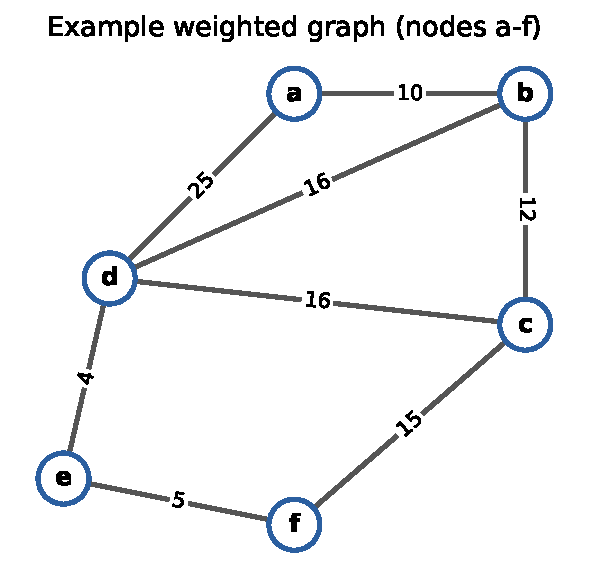
\includegraphics[width=0.55\textwidth]{fig01_example_graph.pdf}
  \end{center}

  \begin{block}{Reading the graph}
    The path $a \to b$ has cost~10.  The path $a \to d$ has cost~25.  From
    $b$ you can reach $c$ with cost~12 or $d$ with cost~16.  Node $d$ connects
    further to $e$ (cost~4), which connects to $f$ (cost~5).  From $c$ to $f$
    costs~15.  The graph is \emph{undirected}: every edge can be traversed in
    either direction.
  \end{block}
\end{frame}

%--------------------------------------------------------------------------
\begin{frame}[allowframebreaks]{Dijkstra's Algorithm --- Concept}
%--------------------------------------------------------------------------
  \textbf{Dijkstra's algorithm} (Dijkstra, 1959) solves the
  \emph{single-source shortest-path problem}: given a starting node, find
  the shortest route from that node to every other node in the graph
  (or, in the modified variant, to a specific finish node).

  \medskip
  The algorithm maintains two labels for every node:
  \begin{itemize}
    \item $d[\,n\,]$ --- the best (shortest) distance found so far from the
      start node to node $n$.  Initially set to $\infty$ for all nodes
      except the start node itself (which has $d = 0$).
    \item $\text{prev}[\,n\,]$ --- the \emph{predecessor} node on the best
      path found so far.  By following the \texttt{prev} labels backwards
      from the finish node, you can reconstruct the actual route.
      Initially \texttt{null} for every node.
  \end{itemize}

  \medskip
  The algorithm also maintains an \emph{unvisited} set containing all nodes
  that have not yet been finalised.

  \begin{block}{Core idea}
    At each iteration, the algorithm picks the unvisited node $c$ with the
    smallest $d[\,c\,]$ (the ``current'' node) and examines all of $c$'s
    neighbours.  For each neighbour $n$, it computes the distance through
    $c$: $\text{distToN} = d[\,c\,] + \text{dist}(c, n)$.  If this is
    better than the previously recorded $d[\,n\,]$, both labels are updated.
    Node $c$ is then removed from the unvisited set.
  \end{block}

  \begin{alertblock}{Why does this work?}
    Because we always process the node with the \emph{smallest} accumulated
    distance first (a greedy choice), once a node is removed from the
    unvisited set its distance is guaranteed to be optimal.  Any future path
    to that node would be longer, because all edge weights are
    non-negative.
  \end{alertblock}

  \framebreak

  \textbf{Algorithm 16 --- Dijkstra (shortest route tree variant).}
  This version computes the shortest path from the start node to
  \emph{all} other nodes, building a complete shortest-path tree.

  \begin{block}{Pseudocode: Dijkstra Flood (Algorithm 16)}
  \begin{enumerate}\setcounter{enumi}{0}
    \item[\footnotesize 1:] \texttt{Procedure Dijkstra(start)}
    \item[\footnotesize 2:] \quad $\text{dists}[\,] \leftarrow \infty$ \hfill
      \textit{// initialise all distances to infinity}
    \item[\footnotesize 3:] \quad $\text{previous}[\,] \leftarrow \text{null}$
    \item[\footnotesize 4:] \quad $\text{current} \leftarrow \text{start}$
    \item[\footnotesize 5:] \quad $\text{dists}[\text{current}] \leftarrow 0$
    \item[\footnotesize 6:] \quad $\text{unvisited} \leftarrow
      \text{Graph.allNodes}()$
    \item[\footnotesize 7:] \quad \textbf{while} $\text{unvisited.size} > 0$
      \textbf{do}
    \item[\footnotesize 8:] \qquad $\text{neighbours} \leftarrow
      \text{Graph.neighbours(current)}$
    \item[\footnotesize 9:] \qquad \textbf{for} Node $n$ in neighbours
      \textbf{do}
    \item[\footnotesize 10:] \quad\qquad $\text{distToN} \leftarrow
      \text{dists[current]} + \text{Graph.dist(current}, n)$
    \item[\footnotesize 11:] \quad\qquad \textbf{if} $\text{distToN} <
      \text{dists}[n]$ \textbf{then}
    \item[\footnotesize 12:] \qquad\qquad $\text{dists}[n] \leftarrow
      \text{distToN}$
    \item[\footnotesize 13:] \qquad\qquad $\text{previous}[n] \leftarrow
      \text{current}$
    \item[\footnotesize 14:] \quad $\text{unvisited.remove(current)}$
    \item[\footnotesize 15:] \quad $\text{current} \leftarrow
      \text{findSmallest(dists, unvisited)}$
  \end{enumerate}
  \end{block}

  \textbf{Line-by-line explanation.}
  Lines~2--5 initialise the data structures: every distance starts at
  $\infty$ except the start node which is~0, and every predecessor is
  \texttt{null}.  Line~6 places every graph node in the unvisited set.
  The \textbf{while} loop on line~7 continues as long as there are
  unvisited nodes.  Lines~8--13 examine all neighbours of the current
  node and update labels when a shorter path is found.  Line~14 marks the
  current node as visited (removes it from the set), and line~15 selects
  the next current node as the one with the smallest distance in the
  unvisited set.
\end{frame}

%--------------------------------------------------------------------------
\begin{frame}[allowframebreaks]{Dijkstra --- Modified Variant (Algorithm 17)}
%--------------------------------------------------------------------------
  The ``flood'' variant (Algorithm~16) is useful when you need the
  distance from one node to \emph{every} other node --- for example when
  pre-computing an Origin-Destination matrix.  However, if you only need
  the distance between two specific nodes, it is wasteful to search the
  entire graph.

  \medskip
  \textbf{Algorithm 17 --- Dijkstra Modified} adds a single early-exit
  check: as soon as the current node equals the finish node, the algorithm
  returns.  Only lines~14--15 differ from Algorithm~16.

  \begin{block}{Pseudocode: Dijkstra Modified (Algorithm 17)}
  \begin{enumerate}\setcounter{enumi}{0}
    \item[\footnotesize 1:] \texttt{Procedure DijkstraMod(start, finish)}
    \item[\footnotesize 2--13:] \textit{(identical to Algorithm 16)}
    \item[\footnotesize 14:] \quad \textbf{if} $(current == finish)$
      \textbf{then return}   \hfill\textit{// early exit}
    \item[\footnotesize 15:] \quad $\text{unvisited.remove(current)}$
    \item[\footnotesize 16:] \quad $\text{current} \leftarrow
      \text{findSmallest(dists, unvisited)}$
  \end{enumerate}
  \end{block}

  \begin{alertblock}{Key insight}
    This modification means the algorithm only searches the part of the
    graph that lies between the start and the finish.  For a large city
    graph, this can reduce the number of nodes examined from tens of
    thousands to a few hundred.
  \end{alertblock}

  \framebreak

  \textbf{Algorithm 18 --- PrintRoute.}  Once Dijkstra has run, the
  \texttt{prev[]} array forms a backwards-linked chain from the finish
  node back to the start.  The following procedure follows that chain to
  print each road name and accumulate the total distance.

  \begin{block}{Pseudocode: PrintRoute (Algorithm 18)}
  \begin{enumerate}\setcounter{enumi}{0}
    \item[\footnotesize 1:] \texttt{Procedure PrintRoute(start, finish, prev)}
    \item[\footnotesize 2:] \quad $\text{dist} \leftarrow 0$
    \item[\footnotesize 3:] \quad $\text{current} \leftarrow \text{finish}$
    \item[\footnotesize 4:] \quad $\text{old} \leftarrow
      \text{previous}[\text{finish}]$
    \item[\footnotesize 5:] \quad \textbf{while} $(\text{current} \neq
      \text{null})$ \textbf{do}
    \item[\footnotesize 6:] \qquad $\text{myWay} \leftarrow
      \text{Graph.getWay(current, old)}$
    \item[\footnotesize 7:] \qquad $\text{print}(\text{myWay.name}())$
    \item[\footnotesize 8:] \qquad $\text{dist} \leftarrow \text{dist} +
      \text{Graph.getDist(old, current)}$
    \item[\footnotesize 9:] \qquad $\text{old} \leftarrow \text{current}$
    \item[\footnotesize 10:] \quad $\text{current} \leftarrow
      \text{previous[current]}$
    \item[\footnotesize 11:] \quad $\text{print}(\text{''Distance = ''} +
      \text{dist})$
    \item[\footnotesize 12:] \texttt{EndProcedure}
  \end{enumerate}
  \end{block}

  The \texttt{while} loop walks backwards from the finish node to the
  start by following \texttt{prev} pointers.  At each step, the road name
  and partial distance are collected.  The result is a human-readable
  turn-by-turn description of the route.
\end{frame}

%--------------------------------------------------------------------------
\begin{frame}[allowframebreaks]{Dijkstra --- Worked Example (Step by Step)}
%--------------------------------------------------------------------------
  We now trace Dijkstra's algorithm on the 6-node graph $(a, b, c, d, e, f)$
  with start~$= a$ and finish~$= f$.  The figure below shows the state of
  the algorithm at each of the six main steps.

  \begin{center}
    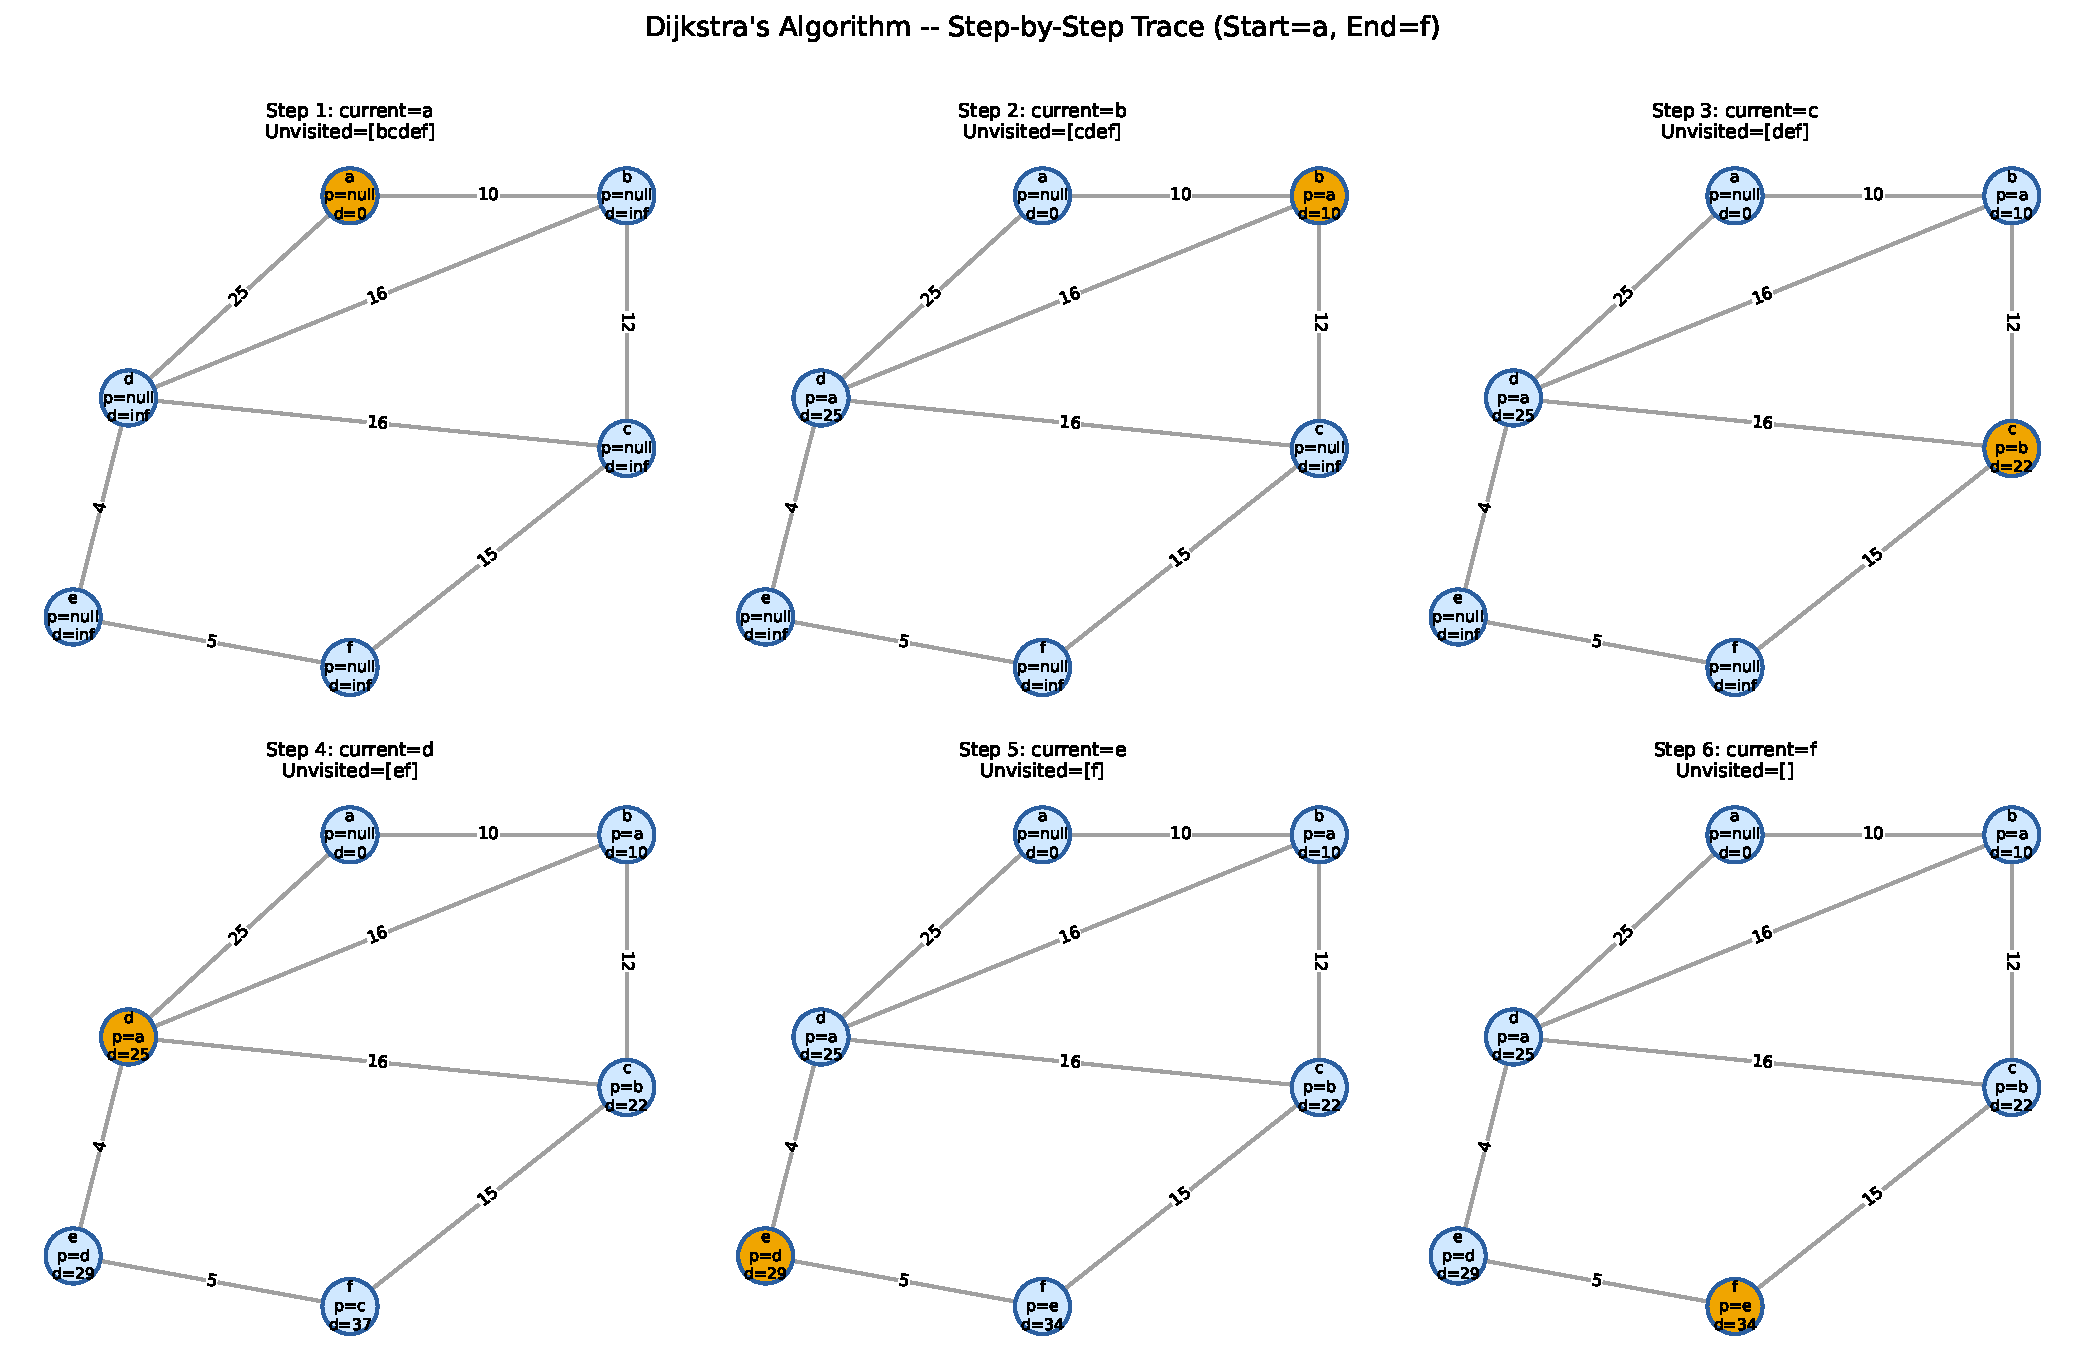
\includegraphics[width=0.90\textwidth]{fig02_dijkstra_steps.pdf}
  \end{center}

  \framebreak

  \textbf{Step-by-step narrative.}

  \begin{exampleblock}{Step 1 --- Initialise, current = $a$}
    $d[a] = 0$, all other distances $= \infty$.  The unvisited set contains
    $\{b,c,d,e,f\}$.  The algorithm examines $a$'s neighbours: $b$ (edge
    weight~10) and $d$ (edge weight~25).  Because $0+10 < \infty$ and
    $0+25 < \infty$, both are updated: $d[b]=10, \text{prev}[b]=a$ and
    $d[d]=25, \text{prev}[d]=a$.
  \end{exampleblock}

  \begin{exampleblock}{Step 2 --- current = $b$ (smallest unvisited distance = 10)}
    Neighbours of $b$: $c$ (weight~12, giving $d[c] = 10+12 = 22$) and $d$
    (weight~16, giving $10+16=26 > 25$, so $d[d]$ is \emph{not} updated).
    Updated: $d[c]=22, \text{prev}[c]=b$.
  \end{exampleblock}

  \begin{exampleblock}{Step 3 --- current = $c$ (dist = 22)}
    Neighbours of $c$: $f$ (weight~15, $22+15=37$) and $d$ (weight~16,
    $22+16=38 > 25$).  Updated: $d[f]=37, \text{prev}[f]=c$.
  \end{exampleblock}

  \begin{exampleblock}{Step 4 --- current = $d$ (dist = 25)}
    Neighbours of $d$: $e$ (weight~4, $25+4=29$).  Updated: $d[e]=29,
    \text{prev}[e]=d$.  ($b$ and $c$ already have smaller distances.)
  \end{exampleblock}

  \framebreak

  \begin{exampleblock}{Step 5 --- current = $e$ (dist = 29)}
    Neighbours of $e$: $f$ (weight~5, $29+5=34 < 37$).  Better route to
    $f$ found!  Updated: $d[f]=34, \text{prev}[f]=e$.
  \end{exampleblock}

  \begin{exampleblock}{Step 6 --- current = $f$ (dist = 34)}
    $f$ is the finish node.  The modified Dijkstra would stop here.
    The shortest route from $a$ to $f$ is:
    \[ a \to d \to e \to f, \quad \text{total distance} = 25+4+5 = 34. \]
    We find this by following the \texttt{prev} chain: $\text{prev}[f]=e$,
    $\text{prev}[e]=d$, $\text{prev}[d]=a$.
  \end{exampleblock}

  \begin{center}
    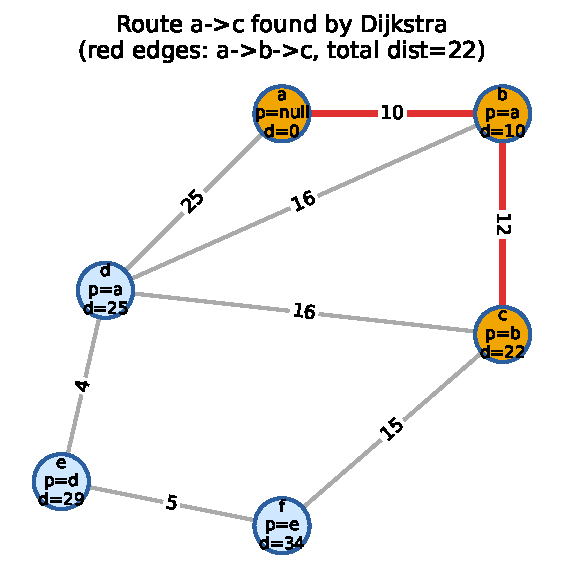
\includegraphics[width=0.48\textwidth]{fig03_dijkstra_route.pdf}
  \end{center}
\end{frame}

%--------------------------------------------------------------------------
\begin{frame}[allowframebreaks]{A* Algorithm --- Concept and Motivation}
%--------------------------------------------------------------------------
  Dijkstra's algorithm has a potential weakness on large graphs: at each
  step it must scan the entire unvisited list to find the node with the
  smallest distance.  More importantly, Dijkstra expands in all directions
  equally from the start --- it does not ``know'' where the finish is.

  \medskip
  \textbf{A*} (pronounced ``A-Star'', Hart et al., 1968) addresses this by
  using a \emph{heuristic} to direct the search towards the finish node.
  Instead of an unvisited list, A* maintains an \textbf{Open List}
  containing only those nodes currently under consideration.

  \begin{block}{The A* Heuristic: $h = d_s + d_e$}
    The priority score $h$ (h) for each node in the open list is:
    \[
      h = d_s + d_e
    \]
    where:
    \begin{itemize}
      \item $d_s$ --- the \emph{known} distance from the start node to
        this node (computed exactly, as in Dijkstra).
      \item $d_e$ --- the \emph{estimated} distance from this node to
        the finish node, computed using the \textbf{Haversine formula}
        (the great-circle distance between two GPS coordinates, treating
        the earth as a sphere).
    \end{itemize}
    The algorithm always picks the node in the open list with the
    \emph{smallest} $h$ as the next current node.
  \end{block}

  \framebreak

  \begin{center}
    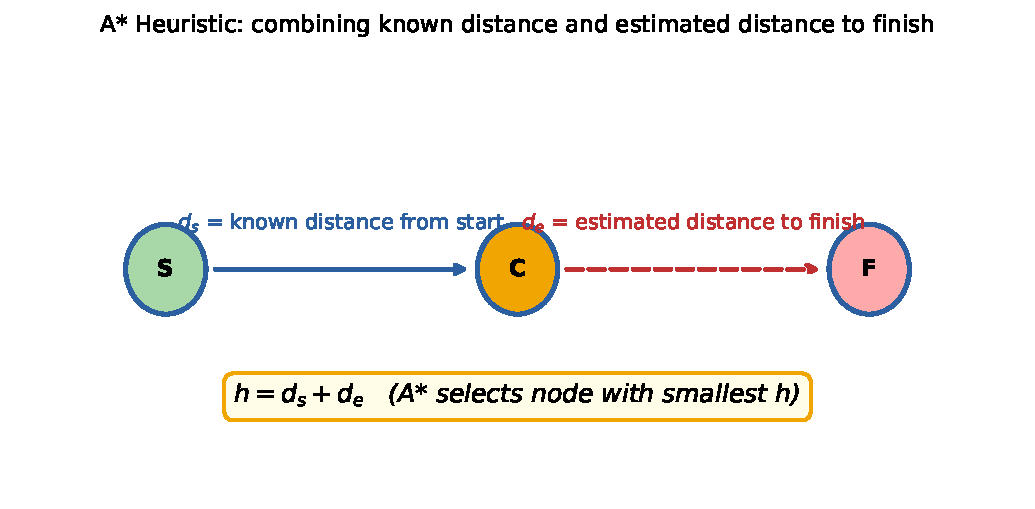
\includegraphics[width=0.75\textwidth]{fig05_astar_heuristic.pdf}
  \end{center}

  \begin{alertblock}{How to read this formula}
    $h$ balances two competing pieces of information: how far we have
    already travelled ($d_s$), and how far we still need to go ($d_e$).
    Choosing the node with the smallest $h$ means we prefer nodes that
    are both \emph{close to the start} (short $d_s$) \emph{and} close to
    the finish (short $d_e$).  This is why A* tends to search in a
    narrow ``corridor'' towards the destination rather than fanning out
    in all directions like Dijkstra.
  \end{alertblock}

  \medskip
  Because the Haversine distance is an \emph{underestimate} of the true
  road distance (roads are rarely straight lines), the heuristic is
  \textbf{admissible}: it never overestimates the true cost.  An
  admissible heuristic guarantees that A* finds the optimal path.

  \framebreak

  \textbf{Algorithm 19 --- A-Star.}

  \begin{block}{Pseudocode: A* (Algorithm 19)}
  \begin{enumerate}\setcounter{enumi}{0}
    \item[\footnotesize 1:] \texttt{Procedure AStar(start, finish)}
    \item[\footnotesize 2:] \quad $\text{dists}[\,] \leftarrow \infty$
    \item[\footnotesize 3:] \quad $\text{previous}[\,] \leftarrow \text{null}$
    \item[\footnotesize 4:] \quad $\text{current} \leftarrow \text{start}$
    \item[\footnotesize 5:] \quad $\text{dists}[\text{current}] \leftarrow 0$
    \item[\footnotesize 6:] \quad $\text{open.add(current)}$
    \hfill\textit{// only start is in open list}
    \item[\footnotesize 7:] \quad \textbf{while} $(\text{open.size} > 0)$
      \textbf{do}
    \item[\footnotesize 8:] \qquad $\text{neighbours} \leftarrow
      \text{Graph.neighbours(current)}$
    \item[\footnotesize 9:] \qquad \textbf{for} Node $n$ in neighbours
      \textbf{do}
    \item[\footnotesize 10:] \quad\qquad $\text{distToN} \leftarrow
      \text{dists[current]} + \text{Graph.dist(current}, n)$
    \item[\footnotesize 11:] \quad\qquad \textbf{if}
      $(\text{distToN} < \text{dists}[n])$ \textbf{then}
    \item[\footnotesize 12:] \qquad\qquad \textbf{if}
      $(\text{!open.contains}(n))$
    \item[\footnotesize 13:] \qquad\qquad\quad $\text{open.add}(n)$
      \hfill\textit{// add to open list if not there}
    \item[\footnotesize 14:] \qquad\qquad $\text{dists}[n] \leftarrow
      \text{distToN}$
    \item[\footnotesize 15:] \qquad\qquad $\text{previous}[n] \leftarrow
      \text{current}$
    \item[\footnotesize 16:] \quad $\text{open.remove(current)}$
    \item[\footnotesize 17:] \quad $\text{current} \leftarrow
      \text{findClosest(dists, open)}$ \hfill\textit{// use heuristic here}
    \item[\footnotesize 18:] \quad \textbf{if} $(\text{current} ==
      \text{finish})$ \textbf{then}
    \item[\footnotesize 19:] \qquad \textbf{return}
  \end{enumerate}
  \end{block}

  \medskip
  The critical difference from Dijkstra is on lines~12--13 (nodes are only
  added to the open list if not already present) and line~17 where the
  \texttt{findClosest} function orders candidates by the heuristic $h =
  d_s + d_e$ rather than by $d_s$ alone.

  \framebreak

  \textbf{Algorithm 20 --- A* heuristic-based selection (\texttt{findClosest}).}

  \begin{block}{Pseudocode: findClosest (Algorithm 20)}
  \begin{enumerate}\setcounter{enumi}{0}
    \item[\footnotesize 1:] \texttt{Procedure findClosest(dists, unvisited)}
    \item[\footnotesize 2:] \quad $\text{closestD} \leftarrow \infty$
    \item[\footnotesize 3:] \quad $\text{closestN} \leftarrow \text{null}$
    \item[\footnotesize 4:] \quad \textbf{for} Node $n$ in unvisited
      \textbf{do}
    \item[\footnotesize 5:] \qquad $\text{estim} \leftarrow
      \text{dists}[n] + \text{EuclideanDist}(n, \text{finish})$
    \item[\footnotesize 6:] \qquad \textbf{if} $(\text{estim} <
      \text{closestD})$ \textbf{then}
    \item[\footnotesize 7:] \qquad\quad $\text{closestD} \leftarrow
      \text{estim}$
    \item[\footnotesize 8:] \qquad\quad $\text{closestN} \leftarrow n$
    \item[\footnotesize 9:] \quad \textbf{Return} closestD
  \end{enumerate}
  \end{block}

  This procedure loops over all nodes in the open list and computes $h =
  d_s + d_e$ for each (where $d_e$ is approximated by the Euclidean
  straight-line distance to the finish, which is the Haversine formula on
  real geographic data).  The node with the lowest $h$ is returned as the
  next current node.
\end{frame}

%--------------------------------------------------------------------------
\begin{frame}[allowframebreaks]{A* --- Worked Example (Step by Step)}
%--------------------------------------------------------------------------
  We trace A* on the same 6-node graph, with start~$=a$ and finish~$=c$.

  \begin{center}
    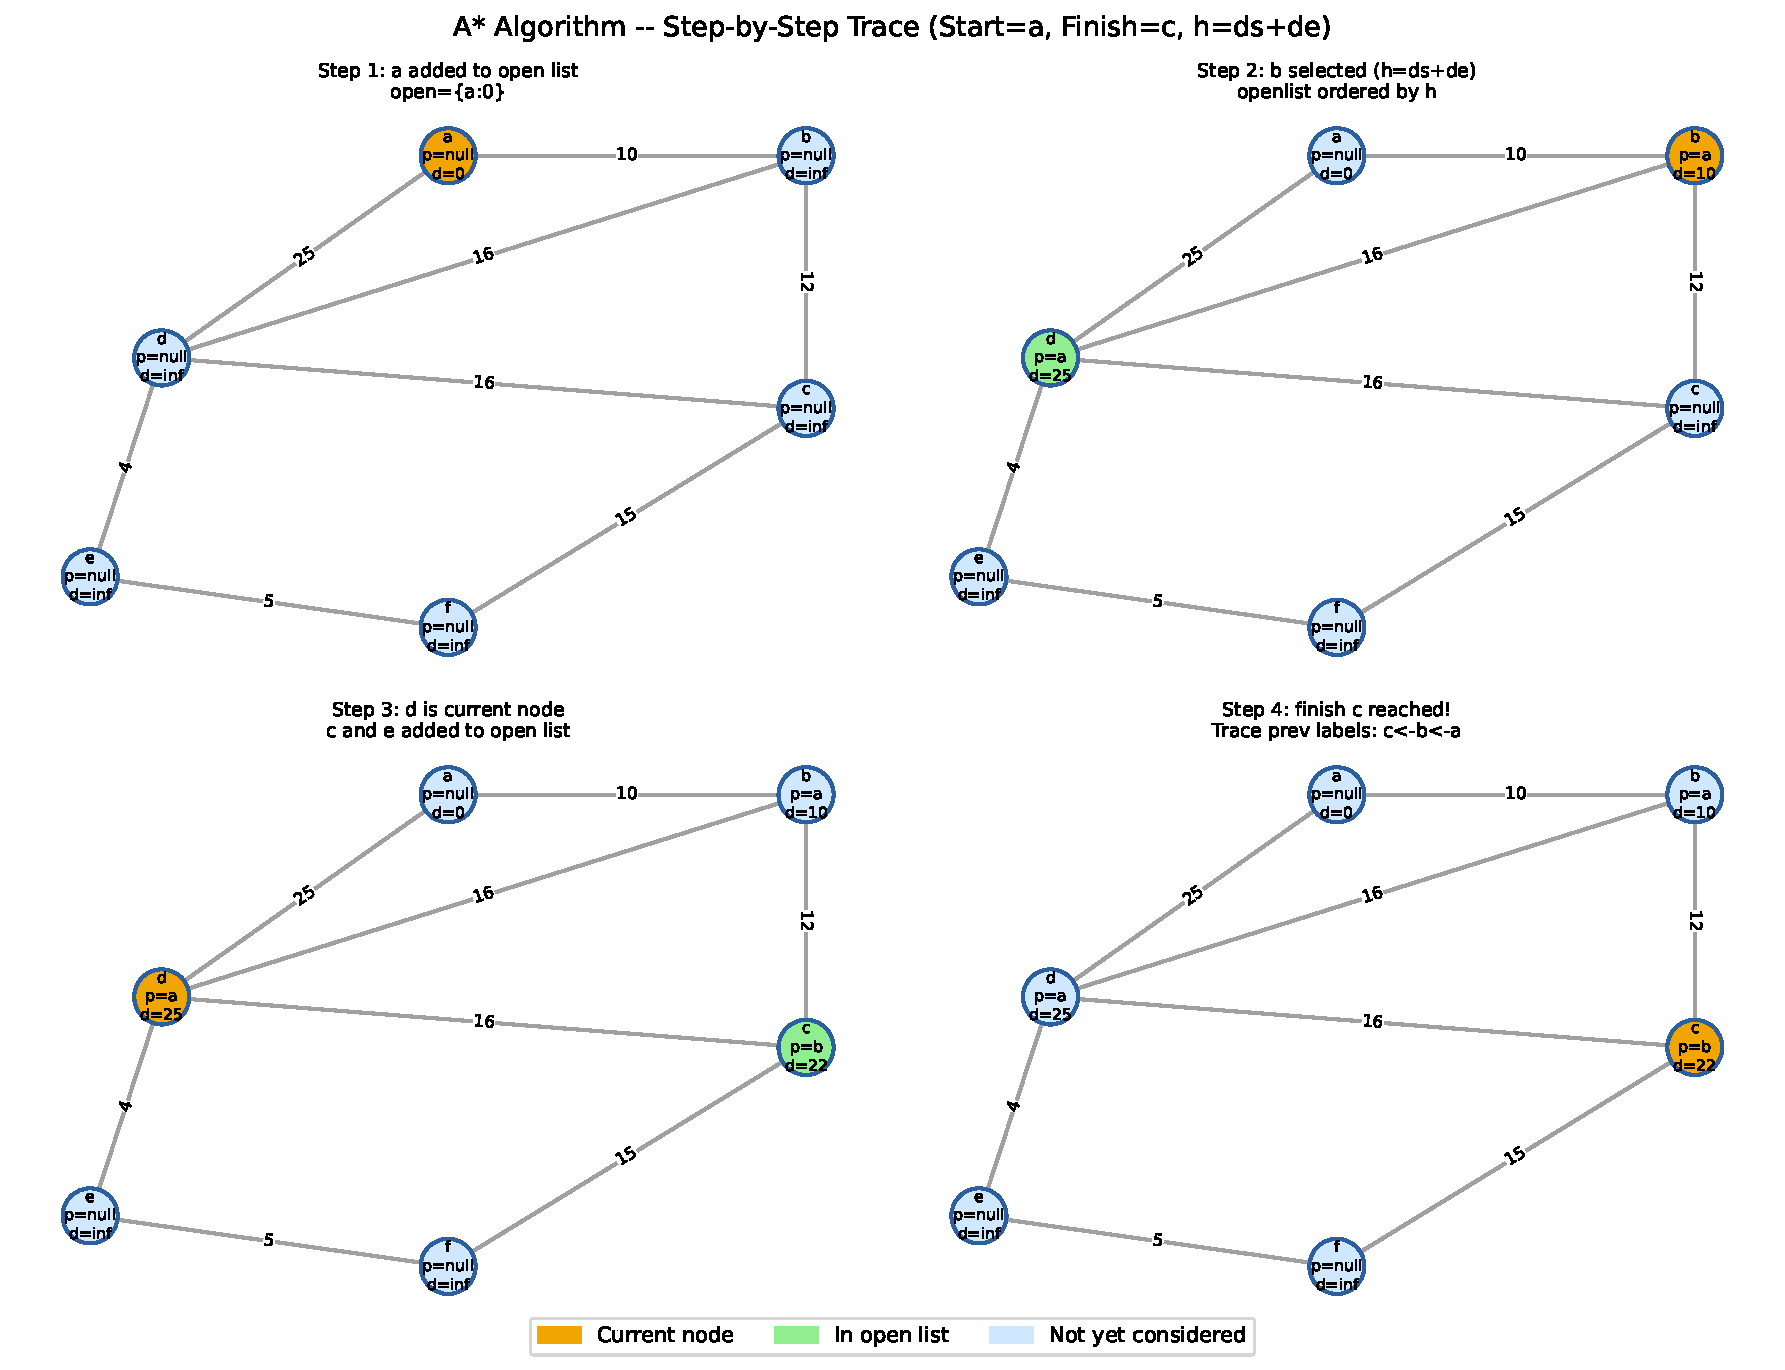
\includegraphics[width=0.85\textwidth]{fig04_astar_steps.pdf}
  \end{center}

  \framebreak

  \textbf{Step-by-step narrative (nodes coloured orange = current,
  green = in open list, blue = not yet considered).}

  \begin{exampleblock}{Step 1 --- Initialise}
    Node $a$ is added to the open list with $d_s=0$.  The heuristic value
    is $h(a) = 0 + d_e(a, c) = d_e(a, c)$.  All other nodes have $d_s=\infty$.
  \end{exampleblock}

  \begin{exampleblock}{Step 2 --- Expand $a$, select next by heuristic}
    $a$'s neighbours $b$ and $d$ are added to the open list.
    $d_s(b) = 10$, $d_s(d) = 25$.  The heuristic scores are:
    $h(b) = 10 + d_e(b,c)$ and $h(d) = 25 + d_e(d,c)$.  Whichever is
    smaller is selected next.  In the book example with the given positions,
    $d$ is selected because its combined score is lower (it lies closer to
    $c$ in the straight-line sense even though its $d_s$ is larger).
  \end{exampleblock}

  \begin{exampleblock}{Step 3 --- Expand current node $d$}
    $d$'s unexplored neighbours ($c$ and $e$) are added to the open list.
    The open list is re-ordered by $h$.  Node $b$ remains in the open list
    from Step~2.
  \end{exampleblock}

  \begin{exampleblock}{Step 4 --- Reach finish $c$}
    When $c$ becomes the current node (either directly via $b$ or via $d$),
    the algorithm returns.  The route is found by tracing \texttt{prev}:
    $\text{prev}[c] = b$, $\text{prev}[b] = a$, giving the path
    $a \to b \to c$ with total distance $10+12=22$.
  \end{exampleblock}

  \begin{alertblock}{Key difference from Dijkstra}
    Dijkstra would have expanded many more nodes (all unvisited nodes with
    distance smaller than 22) before reaching $c$.  A* directed its
    search towards $c$ and expanded far fewer nodes --- at the cost of
    maintaining the open list and computing the heuristic.
  \end{alertblock}
\end{frame}

%--------------------------------------------------------------------------
\begin{frame}[allowframebreaks]{Bidirectional Search}
%--------------------------------------------------------------------------
  Another way to reduce the number of nodes examined is to run
  \emph{two searches simultaneously}: one forward from the start and one
  in reverse from the finish.  When the two search frontiers share a
  common node, a complete route has been found.

  \begin{center}
    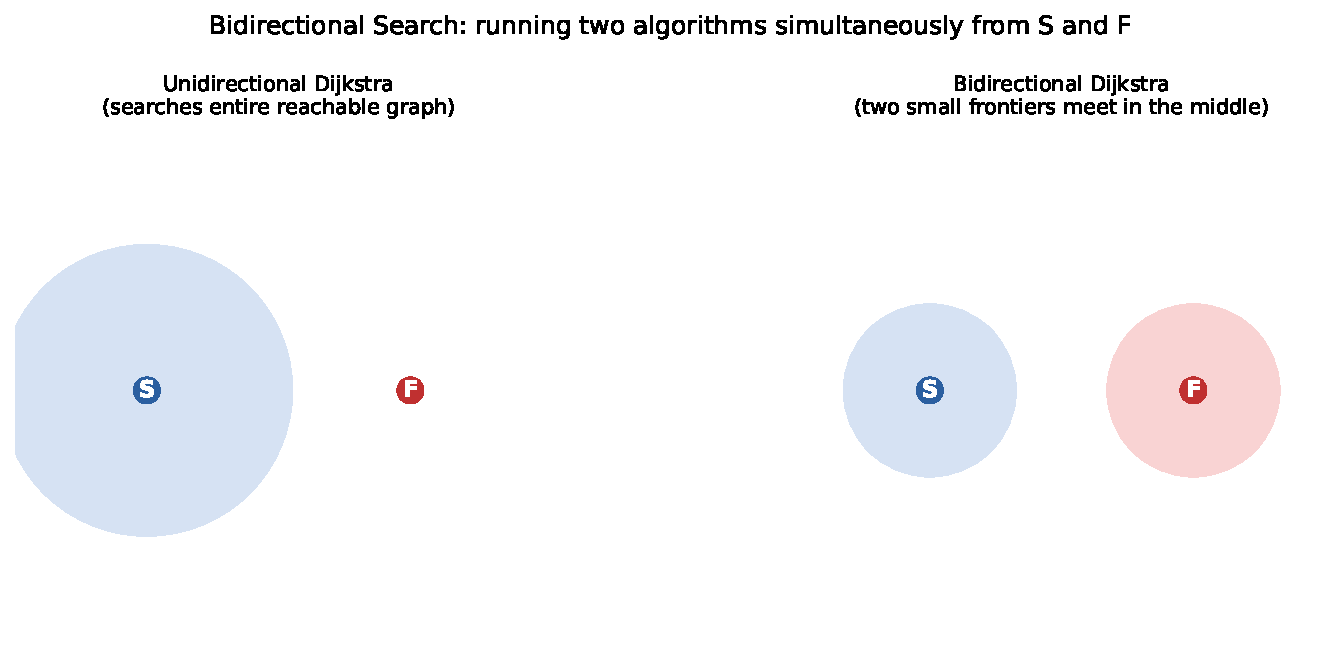
\includegraphics[width=0.80\textwidth]{fig07_bidirectional.pdf}
  \end{center}

  \begin{block}{Principle of Bidirectional Search}
    If the search frontier expands as a circle of radius $r$ in
    unidirectional search, the area searched is $\pi r^2$.  With
    bidirectional search, each frontier only needs radius $r/2$, so
    the total area searched is $2 \times \pi (r/2)^2 = \pi r^2 / 2$
    --- half as much.  For a grid graph, this translates roughly to a
    $\sqrt{2}$ speed-up.
  \end{block}

  \framebreak

  The book implements bidirectional search as the
  \textbf{DijkstraBiDirectional} class.  Two \texttt{Dijkstra} objects
  are created --- one for the forward direction and one for the reverse.
  Both are run one step at a time (using the \texttt{step()} method of
  the abstract \texttt{RoutingAlgorithm} class), and after each pair of
  steps the algorithm checks whether any node is common to both frontiers.

  \medskip
  From the book (Listing~8.4):
  \begin{itemize}
    \item A \texttt{forward} Dijkstra is initialised from \texttt{start}.
    \item A \texttt{reverse} Dijkstra is initialised from \texttt{finish}.
    \item Each iteration calls \texttt{forward.step()} and
      \texttt{reverse.step()}, which return the list of nodes currently
      being considered.
    \item If the intersection of these two lists is non-empty, a common node
      \texttt{join} has been found.  Both algorithms are directed to stop
      at \texttt{join}, and the two half-routes are joined together.
  \end{itemize}

  \begin{alertblock}{Benefit and limitation}
    Bidirectional Dijkstra is particularly effective on large, uniform
    graphs.  The savings are less dramatic with A*, because the heuristic
    already focuses the search.  An \texttt{AStarBiDirectional} class is
    also implemented in the book following the same pattern.
  \end{alertblock}
\end{frame}

%==========================================================================
\section{8.2 A Comparison of Basic Search Algorithms}
%==========================================================================

%--------------------------------------------------------------------------
\begin{frame}[allowframebreaks]{Three Algorithms Under Comparison}
%--------------------------------------------------------------------------
  Section~8.2 compares three routing algorithms on real OpenStreetMap data:

  \begin{block}{The Three Algorithms}
    \begin{itemize}
      \item \textbf{DijkstraFlood} --- Algorithm~16: finds the shortest
        route from the start to \emph{every} node in the graph.  This is
        useful for computing full Origin-Destination (OD) matrices.
      \item \textbf{Dijkstra} --- Algorithm~17: finds the shortest route
        from start to finish, halting as soon as the finish node is
        reached.
      \item \textbf{A-Star} --- Algorithm~19: uses the heuristic
        $h = d_s + d_e$ (Haversine distance to finish) to focus the
        search, maintaining an open list.
    \end{itemize}
  \end{block}

  \medskip
  Both algorithms are tested on two real road networks:

  \begin{enumerate}
    \item \textbf{Sirmione, Italy}: a small network of \textbf{255 nodes}
      connected by \textbf{60 ways} on a peninsula in Lake Garda.  This is
      used to verify that all algorithms find the same route distances.
    \item \textbf{Edinburgh, UK}: a large urban network of \textbf{63,267
      nodes} connected by \textbf{10,612 ways}.  This is the primary
      performance benchmark.
  \end{enumerate}

  \framebreak

  \textbf{Implementation architecture.}
  The algorithms are structured using object-oriented programming so that
  they can be swapped without changing the application code.

  \begin{itemize}
    \item An abstract class \texttt{RoutingAlgorithm} defines the
      interface: \texttt{findPath()} (calls \texttt{step()} repeatedly),
      \texttt{step()} (one iteration of the algorithm), and utility
      methods such as \texttt{getLocations()} and \texttt{getRoadNames()}.
    \item Both \texttt{Dijkstra} and \texttt{AStar} are subclasses of
      \texttt{RoutingAlgorithm}.
    \item A \texttt{Route} class acts as a \emph{facade}: the application
      creates a \texttt{Route} object, passes it a \texttt{RoutingAlgorithm}
      instance, and calls \texttt{buildRoute()}.  The line
      \texttt{testRoute.buildRoute(new AStar())} can be changed to
      \texttt{new Dijkstra()} without touching any other code.
  \end{itemize}

  \begin{exampleblock}{Worked application code (Listing 8.5)}
    \texttt{Graph myGraph = new Graph("westscot.osm");} \\
    \texttt{Route testRoute = new Route(myGraph, 291781127L, 257927392L);} \\
    \texttt{testRoute.buildRoute(new AStar());} \\
    \texttt{System.out.print("distance," + testRoute.getDist());}
  \end{exampleblock}

  The OSM node IDs (\texttt{291781127L}, \texttt{257927392L}) are the
  64-bit integers used by OpenStreetMap to identify specific junctions in
  the real world.
\end{frame}

%--------------------------------------------------------------------------
\begin{frame}[allowframebreaks]{Parsing OpenStreetMap Data}
%--------------------------------------------------------------------------
  OpenStreetMap (OSM) data is stored in an XML-based format.  Each
  \textbf{Way} element describes a polyline (a sequence of connected
  \textbf{Node} elements) and can represent roads, railways, footpaths,
  coastlines, etc.

  \medskip
  The implementation reads OSM data using the \texttt{BasicOSMParser}
  library.  The key steps are:

  \begin{enumerate}
    \item Parse the \texttt{.osm} XML file into a \texttt{Map} of
      \texttt{Element} objects (line~12 in Listing~8.1).
    \item Filter elements by their ID prefix: IDs beginning with ``W''
      (line~19) are Way elements.  Node elements are identified by a
      different prefix.
    \item For each Way, read its \texttt{highway} attribute (line~32).
      Ways without a \texttt{highway} attribute are discarded (line~34--36),
      as are Ways belonging to highway types we are not interested in (e.g.
      \texttt{cycleway}, \texttt{footway}, \texttt{pedestrian} ---
      line~37--39).
    \item For each accepted Way, create a \texttt{RouterWay} object
      containing the ordered list of \texttt{RouterNode} objects along
      that way.  Add the RouterWay to the Graph.
  \end{enumerate}

  \begin{block}{Why filter highway types?}
    Removing non-vehicle ways (footpaths, cycleways, etc.) reduces the
    graph size significantly, which in turn reduces the memory used and
    speeds up routing queries.  For the Edinburgh dataset, the full OSM
    file would contain many more ways than the 10,612 used.
  \end{block}

  \framebreak

  \textbf{Creating an efficient adjacency structure: the Matrix class.}

  A naive $n \times n$ adjacency matrix for Edinburgh ($n = 63,\!267$)
  would require $63,\!267^2 \approx 4 \times 10^9$ entries --- over 16
  gigabytes of memory assuming 32 bytes per reference.

  \medskip
  The implementation instead uses a \textbf{sparse} adjacency structure
  called \texttt{Matrix}.  Each node has a row in a 2-D array of
  \texttt{NodeWay} objects, where each \texttt{NodeWay} stores a
  neighbour's index and the \texttt{RouterWay} connecting them.  Each row
  is initialised to a default size of 10 (since most junctions connect
  to at most 10 roads) and expanded dynamically if needed.

  \begin{exampleblock}{Memory saving}
    For Edinburgh: $63,\!267 \times 10 \times \text{NodeWay size}
    \approx 2.5$\,MB --- a reduction by a factor of over 6,400 compared
    to the full matrix approach.
  \end{exampleblock}

  \medskip
  The \texttt{Matrix.get(x, y)} method (lines~37--48 of Listing~8.2)
  looks up whether nodes $x$ and $y$ are directly linked.  The
  \texttt{Matrix.getNeighbours(x)} method returns all \texttt{RouterWay}
  objects associated with node~$x$.
\end{frame}

%--------------------------------------------------------------------------
\begin{frame}[allowframebreaks]{Results: Sirmione (Small Graph)}
%--------------------------------------------------------------------------
  Table~8.1 from the book shows the results on the Sirmione graph
  (255 nodes, 60 ways).  Twelve problem instances are tested; each label
  ending in ``R'' is the reverse journey of the corresponding numbered
  problem.

  \begin{center}
    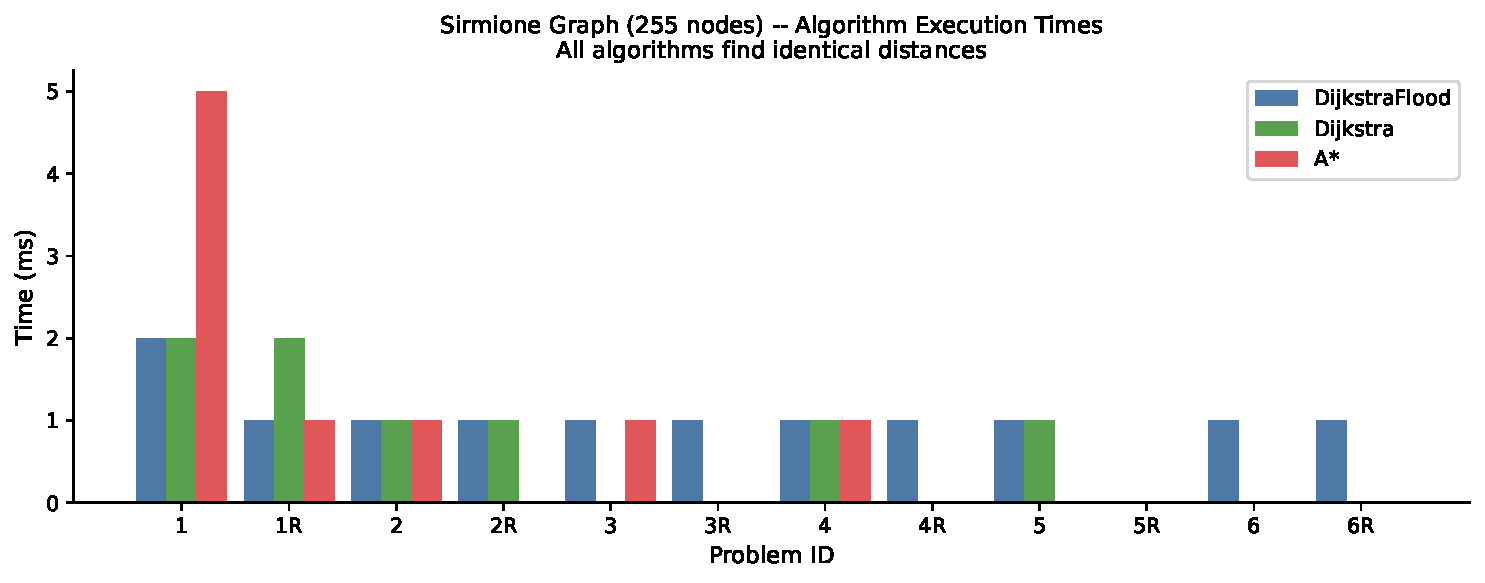
\includegraphics[width=0.75\textwidth]{fig11_sirmione_results.pdf}
  \end{center}

  \framebreak

  \textbf{Key observations from the Sirmione results.}

  \begin{itemize}
    \item \textbf{All algorithms find identical distances.}  This
      confirms correctness: Dijkstra and A* are provably optimal (given
      an admissible heuristic), and on this graph all three methods
      agree on every route length.
    \item \textbf{Execution times are very small} (0--5 ms), confirming
      that on a small graph the choice of algorithm barely matters in
      practice.
    \item \textbf{DijkstraFlood takes 1--2 ms} per query on this graph.
      Since it computes the shortest path to \emph{every} node, running it
      once per node gives a complete OD matrix in total time:
      \[
        t = n \times e = 255 \times 1.5\,\text{ms} \approx 382\,\text{ms}.
      \]
      Here $n$ is the number of nodes and $e$ is the per-run execution
      time.  For a 255-node graph, 382\,ms is perfectly acceptable as a
      one-time pre-computation.
    \item \textbf{A* is occasionally slower} on the small Sirmione graph
      (e.g., problem~1: 5\,ms vs 2\,ms for Dijkstra).  This overhead comes
      from the heuristic computation (Haversine formula) and the open-list
      management, which only pay off on larger graphs.
  \end{itemize}

  \begin{alertblock}{Takeaway from Sirmione}
    For small graphs, all algorithms give equivalent results in negligible
    time.  The important comparison requires a large, real-world graph.
  \end{alertblock}
\end{frame}

%--------------------------------------------------------------------------
\begin{frame}[allowframebreaks]{Results: Edinburgh (Large Graph)}
%--------------------------------------------------------------------------
  The Edinburgh city graph (63,267 nodes, 10,612 ways) provides a
  realistic large-scale benchmark.  Twenty-eight distinct routes are tested
  (each tested in both directions, giving 56 data points).  Each route is
  run 10 times and the average time is recorded.

  \begin{center}
    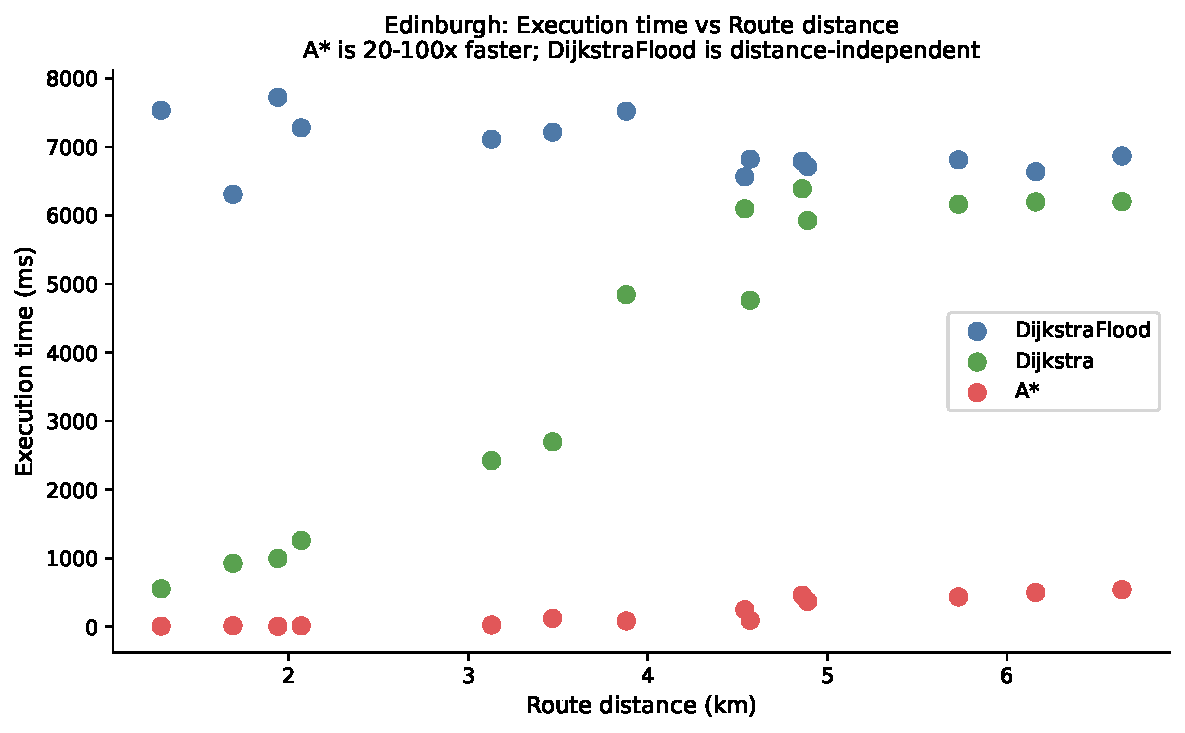
\includegraphics[width=0.85\textwidth]{fig12_edinburgh_scatter.pdf}
  \end{center}

  \framebreak

  \textbf{Performance summary (Edinburgh dataset).}

  \begin{center}
    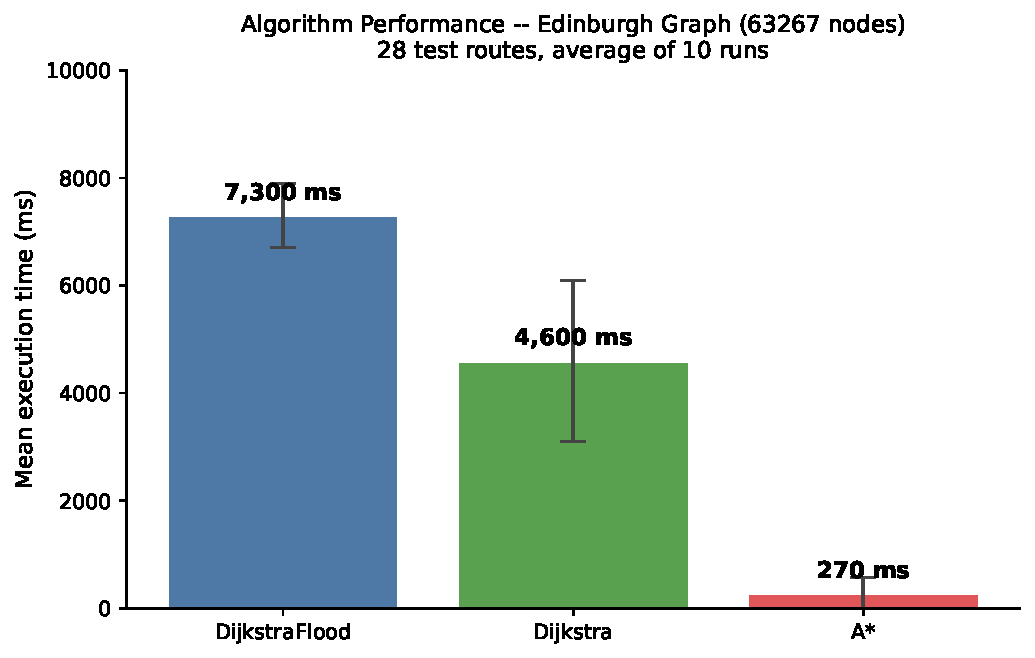
\includegraphics[width=0.75\textwidth]{fig06_performance_comparison.pdf}
  \end{center}

  \textbf{Three striking findings:}

  \begin{enumerate}
    \item \textbf{DijkstraFlood is distance-independent.}  Its execution
      time is always approximately 6,000--9,000\,ms regardless of the
      route distance.  This makes sense: it always searches the entire
      graph of 63,267 nodes.  The variation between runs is caused by the
      Java garbage collector and operating-system scheduling, not by the
      algorithm itself.

    \item \textbf{Dijkstra correlates with distance.}  The modified Dijkstra
      (which halts at the finish) shows a clear positive correlation between
      route length and execution time: longer routes require more of the
      graph to be searched.

    \item \textbf{A* is dramatically faster.}  For the same 28 routes,
      A* times range from under 10\,ms to about 1,258\,ms --- typically
      \textbf{20 to 100 times faster} than Dijkstra.  A* finds the
      same route distances as Dijkstra (no statistically significant
      difference, $p=1.0$ in a T-test).
  \end{enumerate}

  \framebreak

  \begin{block}{Statistical analysis}
    A T-test is used to determine whether the route distances found by
    different algorithms are statistically different.  A T-test value
    $p > 0.9$ means we cannot reject the hypothesis that the algorithms
    produce the same distances.  The book reports:
    \begin{itemize}
      \item DijkstraFlood vs.\ Dijkstra: $p = 9.571$ (same distances).
      \item DijkstraFlood vs.\ A*: $p = 1.0$ (identical distances).
    \end{itemize}
    All three algorithms are therefore \emph{equally correct}; they differ
    only in \emph{speed}.
  \end{block}

  \begin{alertblock}{Why A* is faster on urban graphs}
    Edinburgh's road network is relatively dense and isotropic (roads
    go in many directions).  A* tends to search in a narrow corridor
    towards the destination using the Haversine heuristic.  The result is
    that A* visits far fewer nodes than Dijkstra, which saves time
    proportional to the number of nodes skipped.
  \end{alertblock}

  \begin{exampleblock}{Practical implication}
    When building a vehicle routing solver that evaluates thousands of
    candidate routes per second, replacing Dijkstra with A* can provide
    a 20--100$\times$ speed-up with no loss of solution quality.
  \end{exampleblock}
\end{frame}

%--------------------------------------------------------------------------
\begin{frame}[allowframebreaks]{The Origin-Destination (OD) Matrix}
%--------------------------------------------------------------------------
  A common requirement in logistics is to pre-compute all pairwise
  distances between $n$ locations.  The result is an $n \times n$
  \emph{Origin-Destination (OD) matrix} where entry $[i,j]$ holds the
  shortest road distance from location $i$ to location $j$.

  \begin{center}
    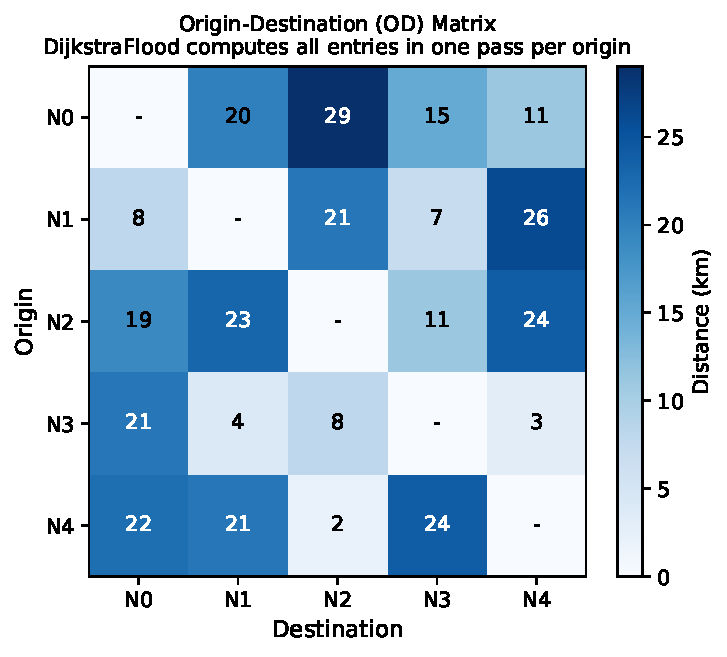
\includegraphics[width=0.45\textwidth]{fig13_od_matrix.pdf}
  \end{center}

  \begin{block}{Computing the OD matrix with DijkstraFlood}
    DijkstraFlood computes the shortest distance from one node to
    \emph{all} other nodes in a single pass.  Running it once for each
    of the $n$ origins fills the entire matrix:
    \[
      t_{\text{total}} = n \times e
    \]
    where $t_{\text{total}}$ is the total time, $n$ is the number of
    nodes, and $e$ is the execution time for one DijkstraFlood run.
    For Sirmione: $255 \times 1.5\,\text{ms} \approx 382\,\text{ms}$,
    which is negligible.
  \end{block}

  Once the OD matrix is computed, routing queries reduce to simple
  table lookups --- far faster than running a routing algorithm at query
  time.  This is the preferred approach when all relevant locations are
  known in advance (e.g., fixed depot and customer locations).
\end{frame}

%==========================================================================
\section{8.3 Hierarchical Structures}
%==========================================================================

%--------------------------------------------------------------------------
\begin{frame}[allowframebreaks]{Motivation for Hierarchical Routing}
%--------------------------------------------------------------------------
  When the graph is very large (e.g., the entire road network of Scotland),
  even A* may be too slow for real-time routing.  The key observation is
  that road networks have a natural \textbf{hierarchy}:

  \begin{itemize}
    \item Long journeys predominantly use \emph{motorways} and \emph{trunk}
      roads for most of their length.
    \item Only the start and end segments use \emph{local} roads
      (residential, unclassified).
  \end{itemize}

  This means we do not need to search the full graph for the bulk of the
  journey --- a much smaller sub-graph of major roads suffices.

  \begin{center}
    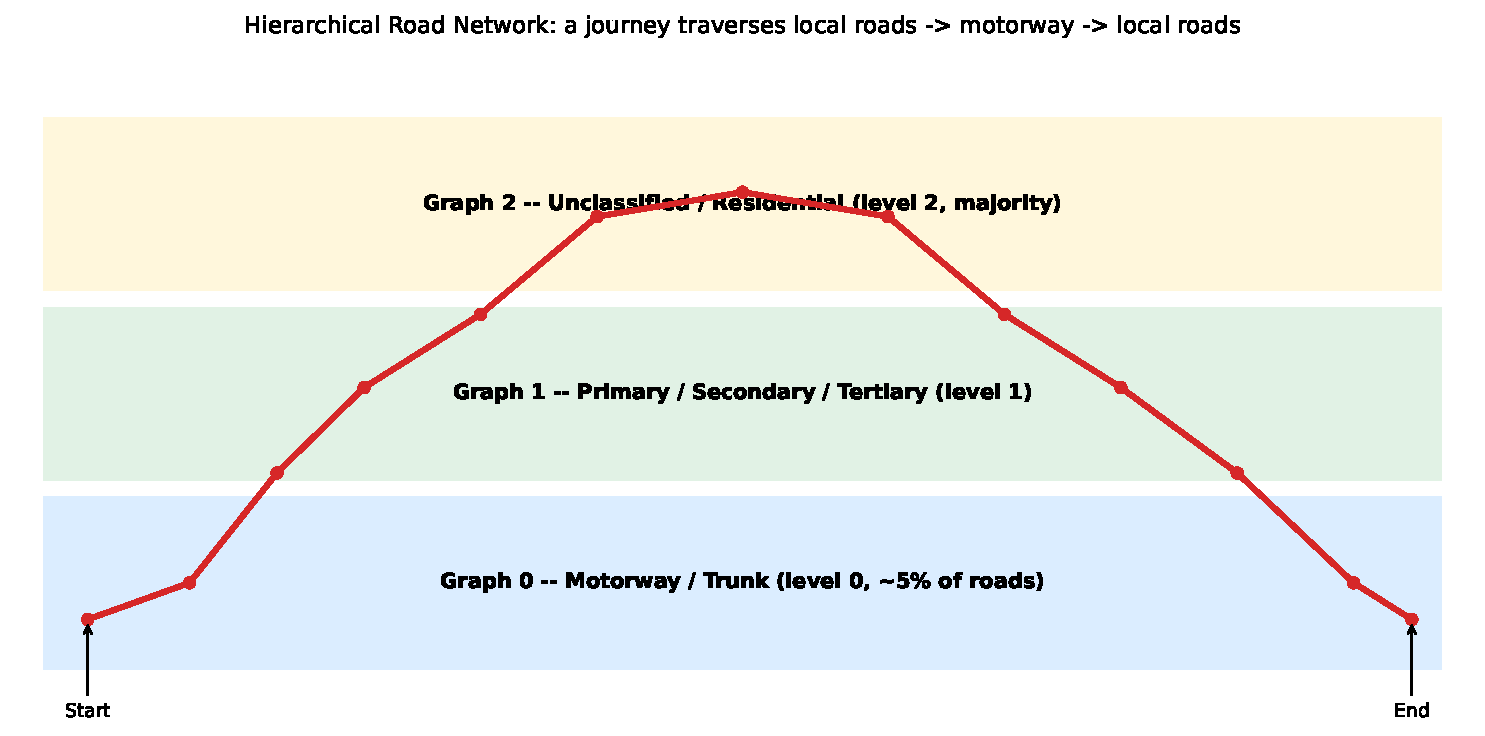
\includegraphics[width=0.80\textwidth]{fig08_hierarchy_structure.pdf}
  \end{center}

  \framebreak

  \textbf{Highway classification in OpenStreetMap.}

  OSM classifies each Way with a \texttt{highway} tag.  The book groups
  these into three tiers:

  \begin{center}
    \begin{tabular}{c l l}
      \toprule
      \textbf{Graph Level} & \textbf{Way types} & \textbf{Purpose} \\
      \midrule
      0 & Motorway, Motorway Link, Trunk, Trunk Link &
          Long-distance backbone \\
      1 & Primary, Secondary, Tertiary &
          Medium-distance connectors \\
      2 & Unclassified, Residential &
          Local access (majority of roads) \\
      \bottomrule
    \end{tabular}
  \end{center}

  The figure below shows the highway classification profile of a journey
  from the centre of Edinburgh to the centre of Glasgow.  Note how the
  bulk of the journey uses motorway-class roads (Graph~0), with only
  short residential sections at each end.

  \begin{center}
    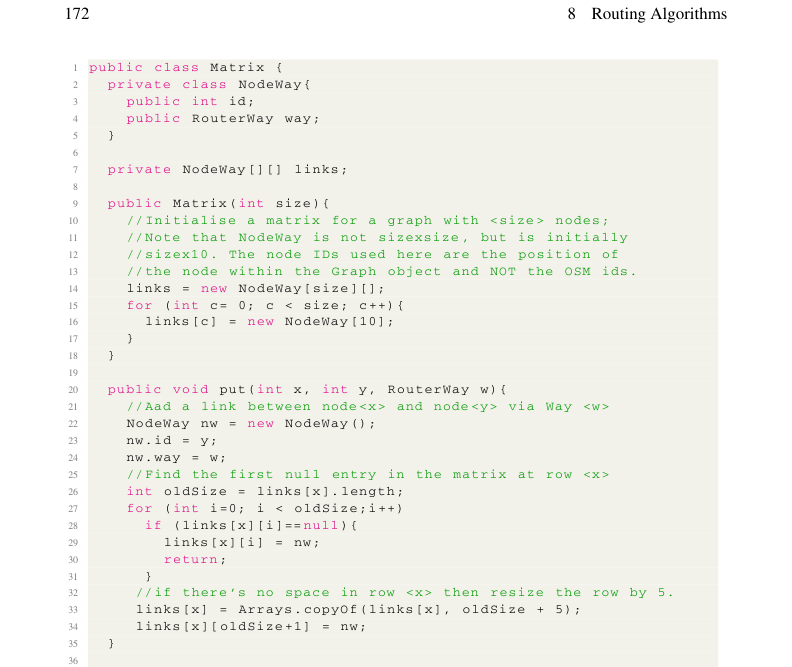
\includegraphics[width=0.80\textwidth]{fig_book_hierarchy_journey.png}
  \end{center}

  \framebreak

  \textbf{Dividing the graph into levels.}

  Instead of one monolithic graph, we maintain an array \texttt{level[]}
  of three graph objects.  Level~0 contains only motorway and trunk ways.
  Level~1 contains primary, secondary, and tertiary ways.  Level~2
  contains all remaining ways.

  \begin{itemize}
    \item Only level~0 is \emph{fully connected} on its own.
    \item Levels~1 and~2 are collections of road segments that are not
      fully connected unless combined with higher levels.
    \item Adjacent levels share \textbf{link nodes}: motorway junctions,
      for instance, appear in both level~0 and level~1.
  \end{itemize}

  \begin{block}{Three advantages of hierarchical graphs}
    \begin{enumerate}
      \item \textbf{Parallelism.} The start-leg and end-leg searches
        (both on level~1) can run on different CPUs simultaneously.
      \item \textbf{Caching.} Frequently used motorway segments (e.g.,
        between major cities) can be cached to avoid recomputation.
      \item \textbf{Graph Size.} No single routing call ever needs to
        search the entire graph.  Level~0 contains only about 5\% of
        all nodes.
    \end{enumerate}
  \end{block}
\end{frame}

%--------------------------------------------------------------------------
\begin{frame}[allowframebreaks]{Hierarchical Routing Algorithm}
%--------------------------------------------------------------------------
  The 3-tier routing algorithm works as follows.  Given a \texttt{start}
  node (in level~2, a local road) and an \texttt{end} node (also in
  level~2), the algorithm assembles the route in three segments:

  \begin{center}
    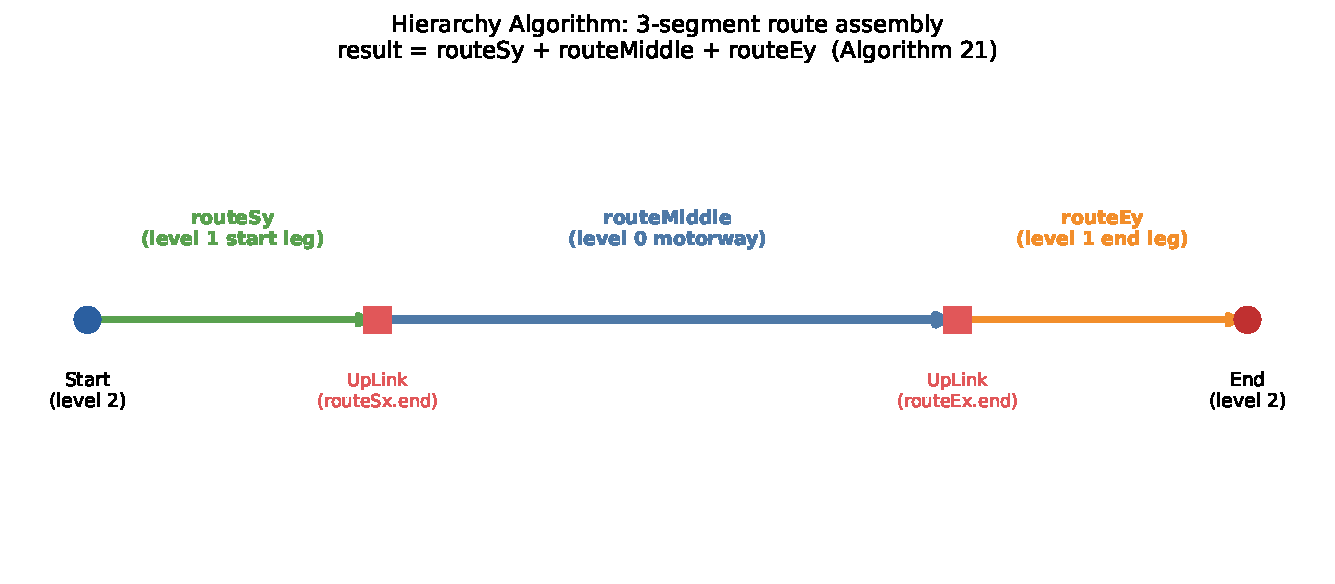
\includegraphics[width=0.80\textwidth]{fig09_hierarchy_route_assembly.pdf}
  \end{center}

  \begin{block}{Algorithm 21 --- Outline Hierarchy Algorithm}
    \begin{enumerate}
      \item \texttt{routeSx = level[2].findLink(start)}
        \hfill \textit{// uplink from level~2 start}
      \item \texttt{routeSy = level[1].findLink(routeSx.end)}
        \hfill \textit{// uplink from level~1 start}
      \item \texttt{routeEx = level[2].findLink(end)}
        \hfill \textit{// uplink from level~2 end}
      \item \texttt{routeEy = level[1].findLink(routeEx.end)}
        \hfill \textit{// uplink from level~1 end}
      \item \texttt{routeMiddle = level[0].path(routeSy.end, routeEy.end)}
        \hfill \textit{// main motorway leg}
      \item \texttt{result = routeSx + routeSy + routeMiddle + routeEy
          + routeEx}
      \item \textbf{Return} result
    \end{enumerate}
  \end{block}

  \framebreak

  \textbf{Explanation of each segment.}

  \begin{itemize}
    \item \textbf{routeSx} is found by running a modified Dijkstra on
      level~2 from the \texttt{start} node until a \emph{link node}
      (a node that also appears in level~1) is reached.  This is called
      \texttt{DijkstraFindUpLink}.

    \item \textbf{routeSy} extends that search upward: from the level~2
      link node, run \texttt{DijkstraFindUpLink} on level~1 until a
      level~0 link node (typically a motorway junction) is found.

    \item \textbf{routeMiddle} is the motorway/trunk leg.  A standard
      Dijkstra (or A*) is run entirely within level~0 from the level~0
      entry point to the level~0 exit point.  Because level~0 contains
      only $\approx 5\%$ of all nodes, this search is very fast.

    \item \textbf{routeEy} and \textbf{routeEx} mirror the start legs,
      working backwards from the end node up to the motorway and then
      back down to the destination.

    \item The five segments are assembled into a \texttt{MultiRoute}
      object, with reversal flags applied to the end legs (which were
      found by searching from the end, not the start).
  \end{itemize}

  \begin{alertblock}{Special case: start and end in same area}
    If the level~1 uplink nodes from start and end happen to be the
    same node (i.e., start and end are close to each other), no level~0
    motorway search is needed.  The algorithm detects this and simply
    runs A* directly on level~1 between the two link nodes.
  \end{alertblock}
\end{frame}

%--------------------------------------------------------------------------
\begin{frame}[allowframebreaks]{Java Implementation of Hierarchical Routing}
%--------------------------------------------------------------------------
  The \texttt{HierarchyTest} class (Listing~8.8) demonstrates the 2-tier
  implementation.  It creates the two graph levels, then runs 100 random
  route queries.

  \medskip
  \textbf{Setting up the levels (Listing~8.7):}

  \begin{block}{Level 0 --- Motorway/Trunk only}
    Level~0 is constructed by loading the OSM file and filtering to
    include \emph{only} \texttt{motorway}, \texttt{motorway\_link},
    \texttt{trunk}, and \texttt{trunk\_link} way types.  This creates a
    small but fully connected backbone graph.
  \end{block}

  \medskip
  \textbf{The \texttt{buildRoute} method (Listing~8.9):}

  \begin{itemize}
    \item Lines~9--11: find the first uplink segment in level~1 by running
      \texttt{DijkstraFindUpLink} from the start node.
    \item Lines~12--15: find the last uplink segment in level~1 from the end.
    \item Lines~16--21: if both uplinks lead to the same level~0 node,
      the start and end are in the same local area.  A direct A* route
      is computed on level~1.
    \item Lines~23--26: otherwise, the middle segment is computed on level~0
      using standard Dijkstra between the two uplink end-points.
    \item Lines~28--33: the three segments are assembled into a
      \texttt{MultiRoute} object and returned.
  \end{itemize}

  \framebreak

  \textbf{Results: Edinburgh to Aberdeen (Fig.\ 8.11).}

  The 2-tier hierarchy produces a 3-part route for this $\approx 200$\,km
  journey:

  \begin{enumerate}
    \item \textbf{Start leg (level~1)}: a short stretch of local roads in
      Edinburgh to the nearest motorway junction.
    \item \textbf{Middle leg (level~0)}: the majority of the journey along
      the A90/A956 motorway/trunk road network.
    \item \textbf{End leg (level~1)}: local roads in Aberdeen from the
      motorway exit to the destination.
  \end{enumerate}

  \begin{center}
    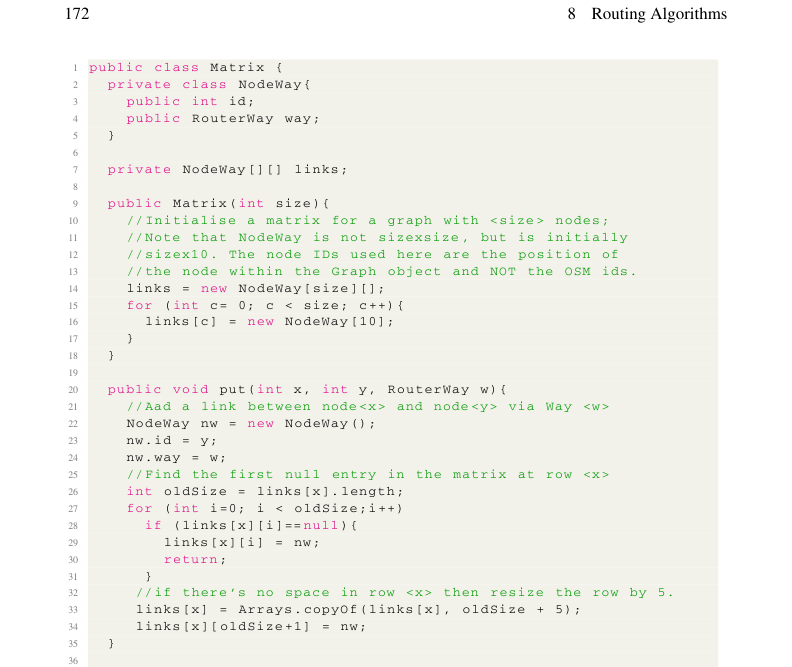
\includegraphics[width=0.65\textwidth]{fig_book_hierarchy_journey.png}
  \end{center}

  \framebreak

  \textbf{Graph size comparison by level.}

  \begin{center}
    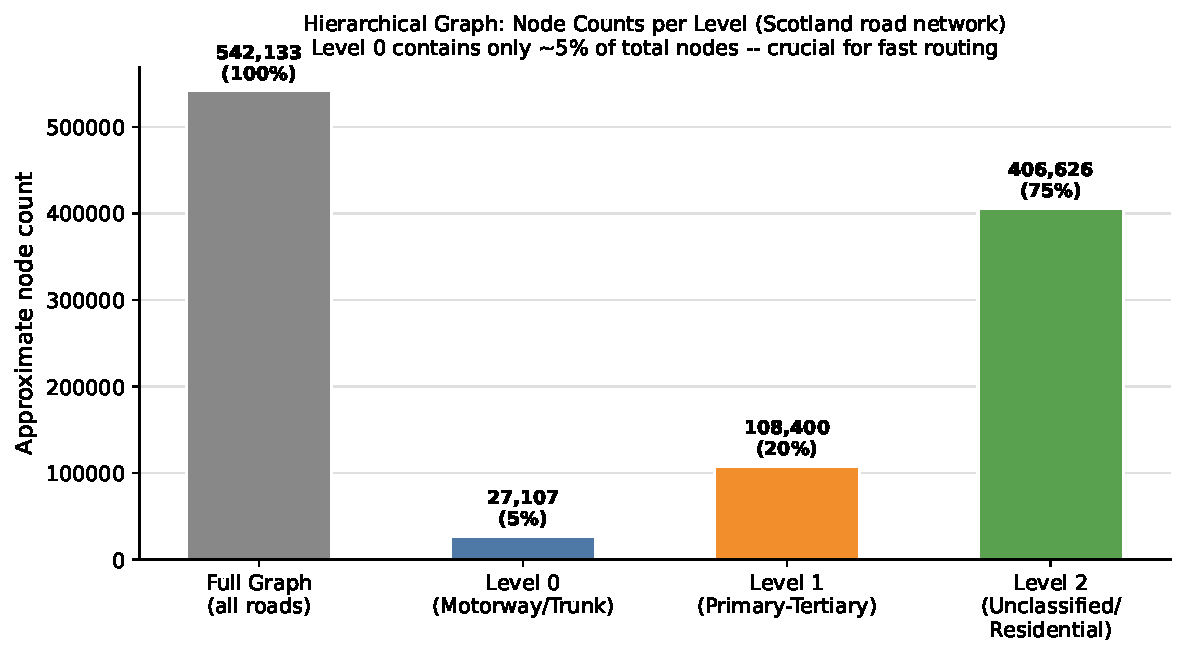
\includegraphics[width=0.75\textwidth]{fig09_graph_sizes.pdf}
  \end{center}

  Level~0 (motorway + trunk) contains only approximately 5\% of the total
  nodes in the Scotland road network.  This means that the most expensive
  search --- the long-distance middle leg --- operates on a graph roughly
  20 times smaller than the full graph.  The start and end legs are on
  local sub-graphs that are also much smaller than the full network.

  \begin{alertblock}{Key takeaway: hierarchical graphs scale}
    For national-scale routing (e.g., all of Scotland with millions of
    nodes), flat Dijkstra and even A* would be too slow for real-time
    queries.  Hierarchical routing solves this by ensuring each sub-query
    operates on a small fraction of the total graph.
  \end{alertblock}
\end{frame}

%--------------------------------------------------------------------------
\begin{frame}[allowframebreaks]{Graph Size and Memory}
%--------------------------------------------------------------------------
  The book analyses the sizes of the graphs created for the
  Edinburgh-to-Aberdeen example (Table~8.5).  Approximately:

  \begin{itemize}
    \item \textbf{Level~0} contains roughly 5\% of the full node count.
      For Scotland as a whole, this still represents a non-trivial graph,
      but it is manageable.
    \item \textbf{Level~1} adds primary, secondary, and tertiary roads,
      bringing the total to roughly 30--40\% of all nodes.
    \item \textbf{Level~2} (the full graph) contains 100\% of nodes.
  \end{itemize}

  \begin{center}
    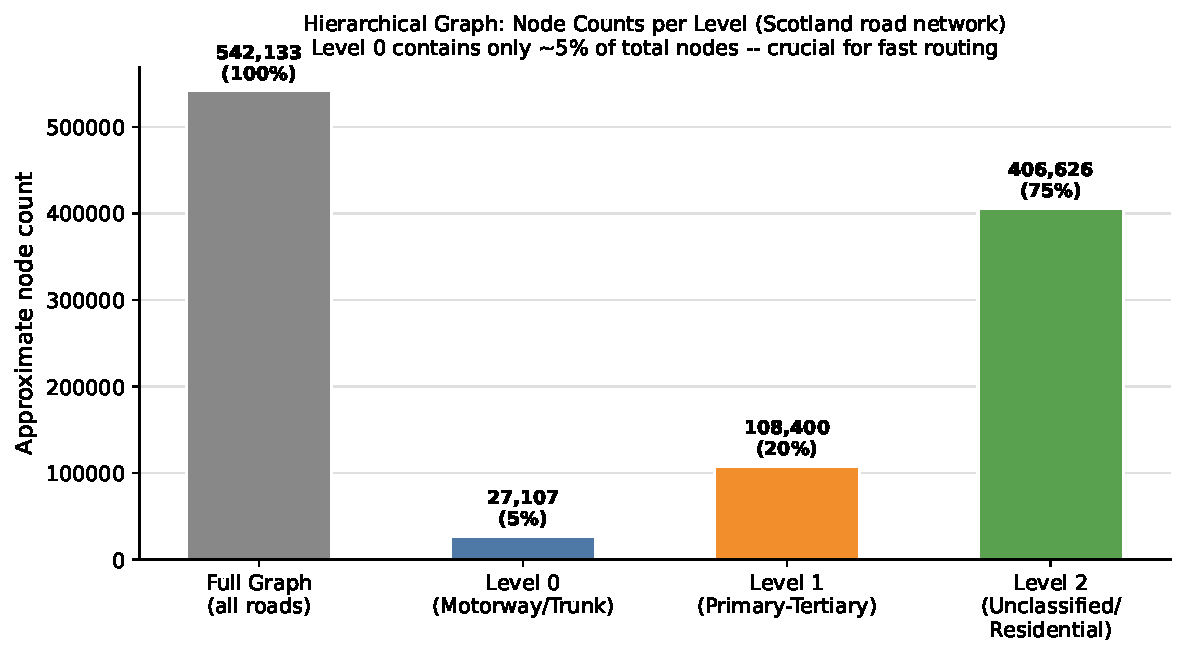
\includegraphics[width=0.70\textwidth]{fig09_graph_sizes.pdf}
  \end{center}

  \begin{block}{Implication for the OSMFilter tool}
    Before loading the OSM data, the \texttt{OSMFilter} utility (Weber,
    2020) is used to remove all non-road data from the OSM file.  This
    reduces parsing time and memory consumption significantly.  For a
    country-scale OSM file, the raw data can be many gigabytes; filtering
    to roads only brings this down to a manageable size.
  \end{block}
\end{frame}

%==========================================================================
\section{8.4 Conclusions}
%==========================================================================

%--------------------------------------------------------------------------
\begin{frame}[allowframebreaks]{Summary and Conclusions}
%--------------------------------------------------------------------------
  This chapter has examined the algorithms needed to find shortest routes
  through road networks, progressing from classical graph search to
  hierarchical multi-graph approaches capable of scaling to national-level
  networks.

  \begin{block}{Summary of Routing Algorithms}
    \begin{center}
      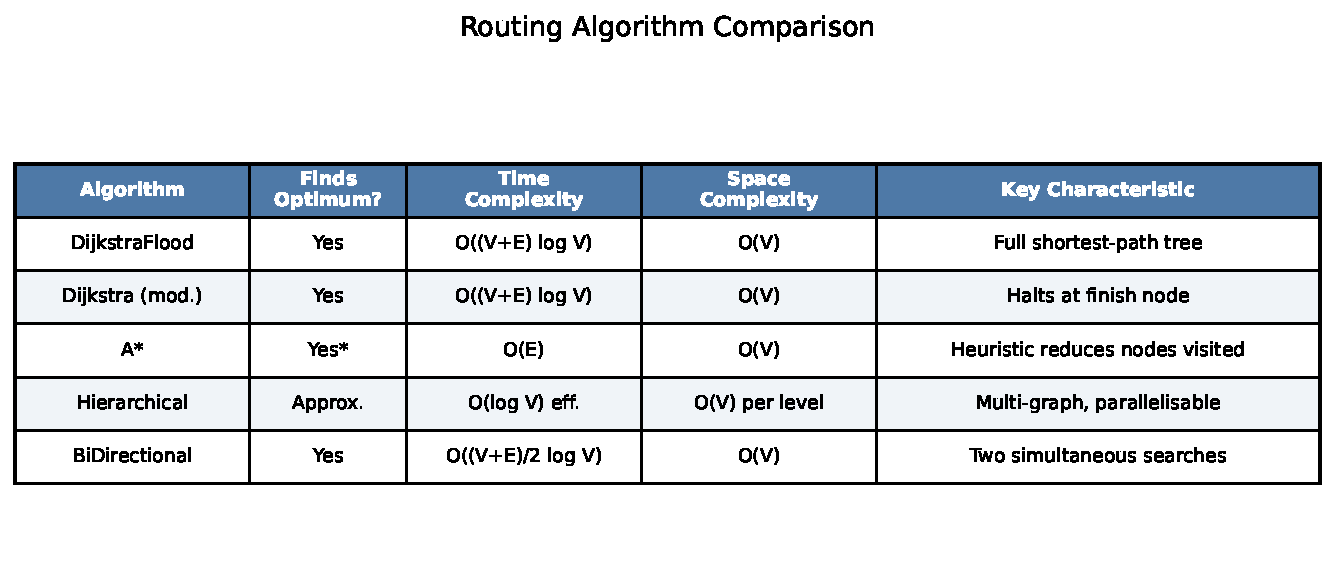
\includegraphics[width=0.90\textwidth]{fig10_complexity_table.pdf}
    \end{center}
  \end{block}

  \framebreak

  \textbf{Key conclusions from the chapter.}

  \begin{enumerate}
    \item \textbf{All three basic algorithms (DijkstraFlood, Dijkstra, A*)
      find identical routes} on real urban road networks (Edinburgh,
      T-test $p = 1.0$).  The choice of algorithm affects speed, not
      solution quality.

    \item \textbf{A* is typically 20--100 times faster than Dijkstra} on
      large urban graphs, because the Haversine heuristic restricts the
      search to a narrow corridor towards the destination.

    \item \textbf{DijkstraFlood is best for pre-computing OD matrices.}
      Its constant time per run means the full matrix can be built in
      $O(n)$ runs, and subsequent distance lookups are $O(1)$ table
      accesses.

    \item \textbf{Hierarchical routing is necessary for national-scale
      networks.}  By splitting the graph into motorway (5\% of nodes),
      main-road, and local-road sub-graphs, the routing algorithm only
      ever searches a small fraction of the total graph for any given
      query.  Additional benefits include parallelism and caching.

    \item \textbf{Bidirectional search} (running forward from start and
      reverse from finish simultaneously) roughly halves the number of
      nodes searched and can be applied to both Dijkstra and A*.
  \end{enumerate}

  \framebreak

  \begin{alertblock}{Implications for delivery problem solvers}
    When a TSP or VRP solver iteratively evaluates millions of candidate
    routes, the routing engine is called for every distance query.
    Choosing the right routing algorithm has a multiplicative effect on
    the solver's overall performance:
    \begin{itemize}
      \item For small instances ($\leq$ a few hundred nodes): Dijkstra
        or DijkstraFlood with an OD matrix is sufficient.
      \item For medium instances on city graphs: A* is preferred.
      \item For national or continental routing: hierarchical techniques
        (or commercial alternatives such as GraphHopper or OpenRouteService,
        which implement Contraction Hierarchies) are necessary.
    \end{itemize}
  \end{alertblock}

  \begin{block}{Further reading}
    \begin{itemize}
      \item Dijkstra, E.W. (1959). A note on two problems in connexion
        with graphs. \textit{Numerische Mathematik}, 1(1), 269--271.
      \item Hart, P.E., Nilsson, N.J., Raphael, B. (1968). A formal
        basis for the heuristic determination of minimum cost paths.
        \textit{IEEE Trans.\ Systems Science and Cybernetics}, 4(2),
        100--107.
      \item Geisberger et al. (2008). Contraction hierarchies: Faster and
        simpler hierarchical routing. \textit{Experimental Algorithms},
        319--333.
    \end{itemize}
  \end{block}
\end{frame}

%==========================================================================
\section{Python Implementation}
%==========================================================================

%--------------------------------------------------------------------------
\begin{frame}[fragile]{Python: Graph Data Structure}
%--------------------------------------------------------------------------
  The following Python code mirrors the Java \texttt{Graph} and
  \texttt{RouterNode} classes from the book.  It provides the three
  interface methods (\texttt{linked}, \texttt{dist}, \texttt{neighbours})
  needed by the routing algorithms.

\begin{lstlisting}[style=pythoncode]
class RouterNode:
    """Represents one OSM node (a junction or point of interest)."""
    def __init__(self, node_id, lat, lon):
        self.node_id = node_id
        self.lat = lat    # latitude in decimal degrees
        self.lon = lon    # longitude in decimal degrees
        self.index = None # position in the graph's node list

class RouterWay:
    """Represents one OSM Way (a road segment connecting two nodes)."""
    def __init__(self, name, nodes, length):
        self.name = name        # road name (e.g. "Princess Street")
        self.nodes = nodes      # list of RouterNode objects
        self.length = length    # total length of the way in metres

class Graph:
    """
    Sparse graph representation of a road network.
    Uses a dictionary of lists (adjacency list) rather than
    a full n x n matrix to save memory.
    """
    def __init__(self):
        self.nodes = {}     # node_id -> RouterNode
        self.adjacency = {} # node_id -> list of (neighbour_id, RouterWay)

    def add_node(self, node):
        self.nodes[node.node_id] = node
        if node.node_id not in self.adjacency:
            self.adjacency[node.node_id] = []

    def add_way(self, way):
        """Add an undirected edge for each consecutive pair of nodes in the way."""
        for i in range(len(way.nodes) - 1):
            n1 = way.nodes[i]
            n2 = way.nodes[i+1]
            # compute edge weight using Haversine distance
            dist = haversine(n1.lat, n1.lon, n2.lat, n2.lon)
            self.adjacency[n1.node_id].append((n2.node_id, dist, way))
            self.adjacency[n2.node_id].append((n1.node_id, dist, way))

    def linked(self, n1_id, n2_id):
        return any(nb == n2_id for nb, _, _ in self.adjacency.get(n1_id, []))

    def dist(self, n1_id, n2_id):
        for nb, d, _ in self.adjacency.get(n1_id, []):
            if nb == n2_id:
                return d
        return None

    def neighbours(self, node_id):
        return [(nb, d) for nb, d, _ in self.adjacency.get(node_id, [])]
\end{lstlisting}
\end{frame}

%--------------------------------------------------------------------------
\begin{frame}[fragile]{Python: Haversine Distance Formula}
%--------------------------------------------------------------------------
  The Haversine formula computes the great-circle distance between two
  points on the Earth's surface given their latitude $\varphi$ (phi,
  degrees north) and longitude $\lambda$ (lambda, degrees east).  It
  accounts for the curvature of the Earth.

  \begin{block}{Haversine Formula}
    \[
      a = \sin^2\!\!\left(\frac{\Delta\varphi}{2}\right)
          + \cos\varphi_1 \cdot \cos\varphi_2 \cdot
            \sin^2\!\!\left(\frac{\Delta\lambda}{2}\right)
    \]
    \[
      d = 2R \cdot \arctan2\!\left(\sqrt{a},\, \sqrt{1-a}\right)
    \]
    where $\Delta\varphi = \varphi_2 - \varphi_1$ (phi, difference in
    latitudes in radians), $\Delta\lambda = \lambda_2 - \lambda_1$
    (lambda, difference in longitudes in radians), and $R \approx
    6,\!371$\,km is the mean Earth radius.
  \end{block}

  \begin{alertblock}{How to read this formula}
    The variable $a$ computes a ``chord length'' intermediate value that
    accounts for both the north-south separation ($\Delta\varphi$) and
    the east-west separation ($\Delta\lambda$, weighted by the cosines of
    the latitudes because longitude lines converge at the poles).  The
    distance $d$ then converts this chord to a surface arc length using
    the radius $R$.  As a point of intuition: two locations at the same
    latitude differ only in $\Delta\lambda$; at the equator
    ($\cos\varphi = 1$) this is maximally effective, while at the poles
    ($\cos\varphi \approx 0$) longitude differences contribute very little.
  \end{alertblock}

\begin{lstlisting}[style=pythoncode]
import math

def haversine(lat1, lon1, lat2, lon2):
    """
    Returns the great-circle distance in metres between two GPS points.
    lat, lon are in decimal degrees.
    """
    R = 6_371_000  # Earth radius in metres
    phi1, phi2 = math.radians(lat1), math.radians(lat2)
    dphi   = math.radians(lat2 - lat1)  # delta phi (latitude difference)
    dlambda = math.radians(lon2 - lon1) # delta lambda (longitude difference)

    a = (math.sin(dphi / 2)**2
         + math.cos(phi1) * math.cos(phi2) * math.sin(dlambda / 2)**2)
    return 2 * R * math.atan2(math.sqrt(a), math.sqrt(1 - a))
\end{lstlisting}
\end{frame}

%--------------------------------------------------------------------------
\begin{frame}[fragile]{Python: Dijkstra's Algorithm (Flood Variant)}
%--------------------------------------------------------------------------
  This implementation finds the shortest distance from \texttt{start} to
  \emph{all} reachable nodes.  It uses a priority queue (min-heap) for
  efficiency --- the standard implementation in Python via
  \texttt{heapq}.

\begin{lstlisting}[style=pythoncode]
import heapq

def dijkstra_flood(graph, start_id):
    """
    Dijkstra flood fill: returns (dists, prev) dicts for all reachable nodes.
    graph   : a Graph object with .neighbours(node_id) method
    start_id: the OSM node ID of the starting node
    """
    # Initialise all distances to infinity
    dists = {node_id: float('inf') for node_id in graph.nodes}
    prev  = {node_id: None         for node_id in graph.nodes}
    dists[start_id] = 0

    # Priority queue entries are (distance, node_id)
    pq = [(0, start_id)]

    while pq:
        current_dist, current = heapq.heappop(pq)

        # Skip if we already found a shorter path (stale entry in heap)
        if current_dist > dists[current]:
            continue

        for neighbour, edge_dist in graph.neighbours(current):
            dist_to_n = dists[current] + edge_dist
            if dist_to_n < dists[neighbour]:
                dists[neighbour] = dist_to_n
                prev[neighbour]  = current
                heapq.heappush(pq, (dist_to_n, neighbour))

    return dists, prev


def get_route(prev, start_id, finish_id):
    """
    Reconstruct the route from start to finish using the prev dictionary.
    Returns a list of node IDs from start to finish.
    """
    route = []
    current = finish_id
    while current is not None:
        route.append(current)
        current = prev[current]
    route.reverse()  # prev chains backwards; reverse to get start->finish order
    if route[0] == start_id:
        return route
    return []  # no path found
\end{lstlisting}
\end{frame}

%--------------------------------------------------------------------------
\begin{frame}[fragile]{Python: Dijkstra Modified (Early Exit)}
%--------------------------------------------------------------------------
  The modified Dijkstra halts as soon as the finish node is popped from
  the priority queue.  This is equivalent to the modified Algorithm~17
  from the book.

\begin{lstlisting}[style=pythoncode]
def dijkstra_mod(graph, start_id, finish_id):
    """
    Modified Dijkstra: stops as soon as finish_id is settled.
    Returns (distance, route_node_ids).
    """
    dists = {node_id: float('inf') for node_id in graph.nodes}
    prev  = {node_id: None         for node_id in graph.nodes}
    dists[start_id] = 0

    pq = [(0, start_id)]

    while pq:
        current_dist, current = heapq.heappop(pq)

        # Early exit: finish node has been settled
        if current == finish_id:
            break

        if current_dist > dists[current]:
            continue  # stale heap entry -- skip

        for neighbour, edge_dist in graph.neighbours(current):
            dist_to_n = dists[current] + edge_dist
            if dist_to_n < dists[neighbour]:
                dists[neighbour] = dist_to_n
                prev[neighbour]  = current
                heapq.heappush(pq, (dist_to_n, neighbour))

    return dists[finish_id], get_route(prev, start_id, finish_id)


# Example usage:
# dist, route = dijkstra_mod(my_graph, start_osm_id, finish_osm_id)
# print(f"Shortest distance: {dist:.0f} m")
# print(f"Route node IDs: {route}")
\end{lstlisting}
\end{frame}

%--------------------------------------------------------------------------
\begin{frame}[fragile]{Python: A* Algorithm}
%--------------------------------------------------------------------------
  The Python A* implementation closely mirrors Algorithm~19 from the book.
  The priority queue orders nodes by $h = d_s + d_e$, where $d_e$ is
  the Haversine distance from the node to the finish.

\begin{lstlisting}[style=pythoncode]
def astar(graph, start_id, finish_id):
    """
    A* algorithm using Haversine great-circle distance as heuristic.
    Returns (distance, route_node_ids).
    """
    finish_node = graph.nodes[finish_id]

    def heuristic(node_id):
        """d_e: Haversine distance from node to finish (underestimate)."""
        n = graph.nodes[node_id]
        return haversine(n.lat, n.lon, finish_node.lat, finish_node.lon)

    dists = {node_id: float('inf') for node_id in graph.nodes}
    prev  = {node_id: None         for node_id in graph.nodes}
    dists[start_id] = 0

    # Priority queue entries: (h_value, node_id)
    # h = d_s + d_e = dists[node_id] + heuristic(node_id)
    open_set = {start_id}
    pq = [(heuristic(start_id), start_id)]

    while pq:
        h_current, current = heapq.heappop(pq)

        if current == finish_id:
            break  # optimal route to finish found

        if current not in open_set:
            continue  # already processed

        open_set.discard(current)

        for neighbour, edge_dist in graph.neighbours(current):
            dist_to_n = dists[current] + edge_dist
            if dist_to_n < dists[neighbour]:
                dists[neighbour] = dist_to_n
                prev[neighbour]  = current
                if neighbour not in open_set:
                    open_set.add(neighbour)
                    h = dist_to_n + heuristic(neighbour)  # h = d_s + d_e
                    heapq.heappush(pq, (h, neighbour))

    return dists[finish_id], get_route(prev, start_id, finish_id)
\end{lstlisting}
\end{frame}

%--------------------------------------------------------------------------
\begin{frame}[fragile]{Python: Comparing Dijkstra vs.\ A*}
%--------------------------------------------------------------------------
  The following demonstration script runs both algorithms on a small
  synthetic graph and compares their results and node-visit counts.

\begin{lstlisting}[style=pythoncode]
import time

def demo_comparison():
    """
    Build a small test graph and compare Dijkstra vs A*.
    This replicates the Sirmione-style experiment from the book.
    """
    # Build a simple 6-node graph matching the book example
    # (nodes assigned approximate GPS coords for heuristic use)
    g = Graph()
    coords = {
        'a': (45.61, 10.60), 'b': (45.61, 10.62),
        'c': (45.60, 10.62), 'd': (45.60, 10.59),
        'e': (45.59, 10.59), 'f': (45.59, 10.61),
    }
    for nid, (lat, lon) in coords.items():
        node = RouterNode(nid, lat, lon)
        node.index = nid
        g.add_node(node)

    # Add edges with synthetic distances (matching book weights x 100m)
    edges = [
        ('a','b',1000), ('a','d',2500), ('b','c',1200), ('b','d',1600),
        ('c','d',1600), ('c','f',1500), ('d','e',400),  ('e','f',500),
    ]
    for u, v, dist_m in edges:
        g.adjacency[u].append((v, dist_m, None))
        g.adjacency[v].append((u, dist_m, None))

    start, finish = 'a', 'f'

    # Run Dijkstra modified
    t0 = time.perf_counter()
    d_dist, d_route = dijkstra_mod(g, start, finish)
    d_time = (time.perf_counter() - t0) * 1000

    # Run A*
    t0 = time.perf_counter()
    a_dist, a_route = astar(g, start, finish)
    a_time = (time.perf_counter() - t0) * 1000

    print(f"Dijkstra: dist={d_dist}m, route={d_route}, time={d_time:.2f}ms")
    print(f"A*:       dist={a_dist}m, route={a_route}, time={a_time:.2f}ms")
    print(f"Same distance? {abs(d_dist - a_dist) < 1e-6}")

if __name__ == '__main__':
    demo_comparison()
\end{lstlisting}
\end{frame}

%--------------------------------------------------------------------------
\begin{frame}[fragile]{Python: Hierarchical Routing (Simplified)}
%--------------------------------------------------------------------------
  A simplified 2-level hierarchical router illustrating the concept
  from Section~8.3.  In practice, levels are separate \texttt{Graph}
  objects loaded with different OSM highway types.

\begin{lstlisting}[style=pythoncode]
def find_uplink(graph, start_id, upper_graph):
    """
    Run Dijkstra from start_id until a node that exists in upper_graph
    is found.  Returns (route_to_link_node, link_node_id).
    This is the 'DijkstraFindUpLink' concept from the book.
    """
    dists = {nid: float('inf') for nid in graph.nodes}
    prev  = {nid: None         for nid in graph.nodes}
    dists[start_id] = 0
    pq = [(0, start_id)]

    while pq:
        d, current = heapq.heappop(pq)
        # Check: is this node a link node (present in the upper graph)?
        if current != start_id and current in upper_graph.nodes:
            route = get_route(prev, start_id, current)
            return dists[current], route, current
        if d > dists[current]:
            continue
        for neighbour, edge_dist in graph.neighbours(current):
            dist_to_n = dists[current] + edge_dist
            if dist_to_n < dists[neighbour]:
                dists[neighbour] = dist_to_n
                prev[neighbour]  = current
                heapq.heappush(pq, (dist_to_n, neighbour))

    return float('inf'), [], None  # no uplink found


def hierarchical_route(level0, level1, start_id, finish_id):
    """
    2-tier hierarchical routing: level1 for local roads, level0 for motorways.
    Returns total distance and assembled route.
    """
    # Find uplinks from start and finish
    d_sx, route_sx, link_s = find_uplink(level1, start_id, level0)
    d_ex, route_ex, link_e = find_uplink(level1, finish_id, level0)

    if link_s is None or link_e is None:
        # Fall back to direct A* on level1
        return astar(level1, start_id, finish_id)

    if link_s == link_e:
        # Start and finish share the same uplink node: no motorway needed
        return astar(level1, start_id, finish_id)

    # Middle leg on level0 (motorway/trunk only -- small graph)
    d_mid, route_mid = dijkstra_mod(level0, link_s, link_e)

    # Assemble total route: start_leg + middle_leg + reversed_end_leg
    total_dist = d_sx + d_mid + d_ex
    full_route = route_sx + route_mid[1:] + list(reversed(route_ex))[1:]
    return total_dist, full_route
\end{lstlisting}
\end{frame}

%--------------------------------------------------------------------------
\begin{frame}[allowframebreaks]{Chapter Summary}
%--------------------------------------------------------------------------
  This chapter has provided the algorithmic foundations needed to find
  routes through real-world road networks, progressing from classical graph
  search algorithms to hierarchical multi-graph techniques.

  \medskip
  \textbf{What you should now be able to do:}

  \begin{enumerate}
    \item \textbf{Describe Dijkstra's algorithm} --- both the flood variant
      that builds a full shortest-path tree and the modified variant that
      halts at a specific finish node.  You should be able to trace the
      algorithm step by step on a small graph.

    \item \textbf{Describe A*} --- how it differs from Dijkstra
      (the Open List and the heuristic $h = d_s + d_e$), why the Haversine
      distance is admissible, and why A* is faster on large graphs.

    \item \textbf{Explain the OD matrix} and why DijkstraFlood is the
      natural algorithm for pre-computing it.

    \item \textbf{Explain hierarchical routing} --- why road networks
      have a natural hierarchy, how splitting the graph by highway type
      enables much faster routing, and the three-segment route assembly
      (local start leg + motorway middle + local end leg).

    \item \textbf{Implement routing in Python} using a priority queue
      (min-heap), and understand the correspondence between the Python
      and Java implementations described in the book.
  \end{enumerate}

  \framebreak

  \textbf{Computational complexity at a glance:}

  \begin{center}
    \begin{tabular}{lcccc}
      \toprule
      \textbf{Algorithm} & \textbf{Optimal?} &
      \textbf{Time} & \textbf{Space} &
      \textbf{When to use} \\
      \midrule
      DijkstraFlood  & Yes  & $O((V+E)\log V)$ & $O(V)$ & OD matrices \\
      Dijkstra (mod) & Yes  & $O((V+E)\log V)$ & $O(V)$ & Single pair \\
      A*             & Yes* & $O(E)$ best case & $O(V)$ & Large graphs \\
      Bidirectional  & Yes  & $\approx O\!\left(\frac{V+E}{2}\log V\right)$
                     & $O(V)$ & Symmetric graphs \\
      Hierarchical   & Approx & $O(\log V)$ eff. & $O(V)$ per level &
                     National scale \\
      \bottomrule
      \multicolumn{5}{l}{\scriptsize * A* is optimal when the heuristic
        is admissible (never overestimates).}
    \end{tabular}
  \end{center}

  \begin{alertblock}{Final message}
    Selecting the right routing algorithm is not just an academic exercise
    --- it directly determines whether a delivery optimisation solver can
    evaluate routes fast enough to be useful in practice.  A* on a city
    graph and hierarchical routing on a national graph are the two most
    important tools in this space.
  \end{alertblock}
\end{frame}

\end{document}
